\chapter[Aplicaciones]{Aplicaciones}

\section{Metodolog\'ia de simulaci\'on de datos y ajuste de los modelos}

Para la elaboraci\'on de este cap\'itulo se ajustaron modelos de diversos cuantiles, a distintos conjuntos de datos. Los datos se obtuvieron de la siguiente manera. Sea $y \in \mathbb{R}$ el valor de la variable de respuesta, $x \in \mathbb{R}$ su respectiva covariable, $g: \mathbb{R} \rightarrow \mathbb{R}$ una funci\'on denominada \textit{tendencia} y $\omega(x) \in \mathbb{R}$ un error aleatorio, se simul\'o
\begin{equation*}
    y = g(x) + \omega(x).
\end{equation*}
Cabe resaltar que se utiliza la notaci\'on $g$, y $\omega$, para diferenciarlas de $f_p$ y $\varepsilon_p$, que son las usadas en el planteamiento de los modelos te\'oricos, vistos en los cap\'itulos anteriores. La raz\'on es que no necesariamente se cumple que $q_p(\omega|x) = 0$. De hecho, como se ver\'a en las siguientes l\'ineas, la funci\'on que se querr\'a estimar no ser\'a $g$, sino las correspondientes $f_p$ para diferentes cuantiles de inter\'es.

La funci\'on real del cuantil $p$\textit{-\'esimo} de $y|x$ se puede obtener como
\begin{equation*}
    q_p(y|x) = g(x) + q_p(\omega|x),
\end{equation*}
funci\'on que en la construcci\'on te\'orica se denomin\'o como $f_p$, y la cual se desea estimar para diversos valores de $p$.

En todos los casos presentados a continuaci\'on se ajust\'o el modelo para el cuantil $0.5$\textit{-\'esimo}, por ser la mediana y una medida de tendencia central alternativa a la media. Tambi\'en se model\'o el cuantil $0.95$\textit{-\'esimo}, ya que es un valor extremo. Finalmente, se busco describir al cuantil $0.25$\textit{-\'esimo}, debido a que el primer cuartil es de inter\'es dentro de algunos contextos, y no es medida de tendencia central, pero tampoco un valor extremo.

Para todos los casos se simularon 60 datos sin reemplazo dentro del intervalo $(-15,15)$, con un refinamiento de 2 decimales. Las razones de elegir esa cantidad de datos, que podr\'ia parecer reducida, fueron varias. Primero, para validar el poder predictivo del algoritmo y su capacidad de ajuste a los valores originales, aún cuando se tienen pocos datos. Segundo, para obtener viabilidad en tiempos de ejecuci\'on, ya que el algoritmo simula en cada iteraci\'on, entre otras variables aleatorias, normales multivariadas y truncadas, con dimensi\'on igual al n\'umero de datos. Dicha simulaci\'on utiliza el m\'etodo de aceptaci\'on y rechazo, por lo que entre mayor sea la dimensi\'on, usualmente requiere de mayor esfuerzo computacional, y, por ende, el tiempo total del ajuste del modelo aumenta de manera significativa. Finalmente, la tercer raz\'on es que esa cantidad de datos permitir\'a observar qu\'e influencia puede tener un dato particular en el ajuste general del modelo.

Una vez simulados los datos, se ajustaron el modelo tradicional de regresi\'on a la media (descrito en la secci\'on \ref{trad_mean_reg} de este trabajo) y el GPDP. Es importante recordar que el primero, adem\'as de ser sobre la media, es lineal en los  par\'ametros de las covariables y con error normal. Por otro lado, el modelo GPDP propone ideas alternativas, como centrar su estimaci\'on en el cuantil de inter\'es, y utilizar componentes no param\'etricos, tanto para modelar la tendencia, como el error. En medio queda una amplia gama de modelos, como el modelo tradicional de regresi\'on sobre cuantiles, o alg\'un modelo de regresi\'on a la media que contemple errores no param\'etricos, por ejemplo. 

Sin embargo, decid\'i realizar esa particular comparaci\'on para descubrir qu\'e tan bueno podr\'ia ser un modelo que contempla ideas alternativas en todas las facetas de la regresi\'on (estad\'istico a modelar, tendencia y error aleatorio), cuando se le comparara con el que utiliza \'unicamente supuestos tradicionales. Eso no significa que si se mezclan algunas ideas alternativas, con algunas tradicionales, no se pueda obtener un tercer modelo, que resulte a\'un mejor. Pero el alcance de esta tesis se limita a comparar \'unicamente esos dos modelos.

Para el ajuste del modelo tradicional se utiliz\'o un poliniomio de orden 5. Es decir, se utilizaron como covariables los valores de $x, x^2, \ldots, x^5$, adem\'as del t\'ermino independiente. A\'un as\'i, dicho ajuste fue simple, computacionalmente hablando, ya que requiri\'o \'unicamente de multiplicaciones matriciales para actualizar sus par\'ametros posteriores. Como par\'ametros iniciales de la distribuci\'on Normal de $\beta$, se utiliz\'o el vector de medias con valores iguales a 0, y como matriz de varianzas y covarianzas, la identidad. En el caso de la \textit{Gamma-Inversa} de $\sigma^2$, el valor de forma usado fue 2, y el de escala, 1.

Por otra parte, el ajuste del GPDP involucr\'o el c\'alculo de una cadena de Markov con ciertas particularidades. En todos los casos se desecharon las primeras $5,000$ simulaciones, para as\'i evitar dependencia de los valores iniciales. Posteriormente, se simularon $15,000$ valores para cada par\'ametro, pero de ellos \'unicamente se guard\'o uno de cada cinco, con la intenci\'on de buscar replicar el comportamiento independiente, que se supone entre los valores. Por lo tanto, se utilizaron $3,000$ valores simulados para aproximar la distribuci\'on posterior de cada par\'ametro. Dicho ajuste se realiz\'o utilizando el paquete \textit{GPDPQuantReg} en R, mismo que, como se detalló en el cap\'itulo anterior, implementa el modelo GPDP para la regresi\'on sobre cuantiles.

Posteriormente, se realiz\'o la predicci\'on para cada $x \in [-15,15]$, tal que $x$ tuviera valor cero para todos los decimales a partir de las cent\'esimas. Es decir, $-15.0,-14.9,\ldots,14.9,15.0$. Se utilizaron ambos modelos para simular $3,000$ predicciones de cada $f_p(x)$ \footnote{El algoritmo utilizado para simular cuantiles del modelo tradicional de regresi\'on a la media se detalla en el \autoref{trad_mean_alg}.}. Posteriormente, se calcularon los cuantiles  muestrales $0.025$ y $0.975$\textit{-\'esimos}, para crear el intervalo de probabilidad al $95\%$ de la estimaci\'on posterior de la predicci\'on. Adem\'as, se calcul\'o el cuantil $0.5$\textit{-\'esimo} (la mediana), para tener una medida de tendencia central de dicha estimaci\'on. 

Finalmente, se obtuvieron m\'etricas que permitieran comparar a grandes rasgos la calidad de estimaci\'on de ambos modelos. Se contrast\'o la estimaci\'on mediana de la predicci\'on con el valor real del cuantil, y se obtuvo el error cuadr\'atico medio, as\'i como la correlaci\'on al cuadrado. Adem\'as se calcul\'o qu\'e porcentaje de los valores reales cayeron dentro del intervalo de probabilidad al 95\%, estimado para la predicci\'on.

\section{Conjuntos de datos simulados}

A continuaci\'on se presentan los diversos conjuntos de datos simulados. Primero, se expone uno que cumple con los supuestos de la regresi\'on tradicional a la media. Posteriormente, se presentan otros que desaf\'ian alguno de sus supuestos, con el fin de comparar c\'omo lidian dicho modelo, y el modelo GPDP, con tal inconveniente. Finalmente, se comparan los resultados.

\subsection{Supuestos tradicionales de regresi\'on a la media}

El primer caso que se presenta es el de un conjunto de datos que se simul\'o con las condiciones com\'unmente supuestas dentro de los modelos de regresi\'on a la media: funci\'on de tendencia polinomial y error normal alrededor de ella, independiente del valor de $x$. Es decir, los errores presentaron homocedasticidad. Expresado en t\'erminos matem\'aticos,
\begin{equation*}
    g(x) = \frac{1}{1000}x^3 - \frac{1}{40}x^2 - \frac{1}{10}x + 6,
\end{equation*}
mientras el error se distribuy\'o $\omega(x) \sim \mathcal{N}(0,1)$. Los datos simulados se pueden observar en la figura \ref{sample_classic}.

\begin{figure}[H]
	\centering
	\caption{Datos simulados con los supuestos tradicionales de regresi\'on.}
	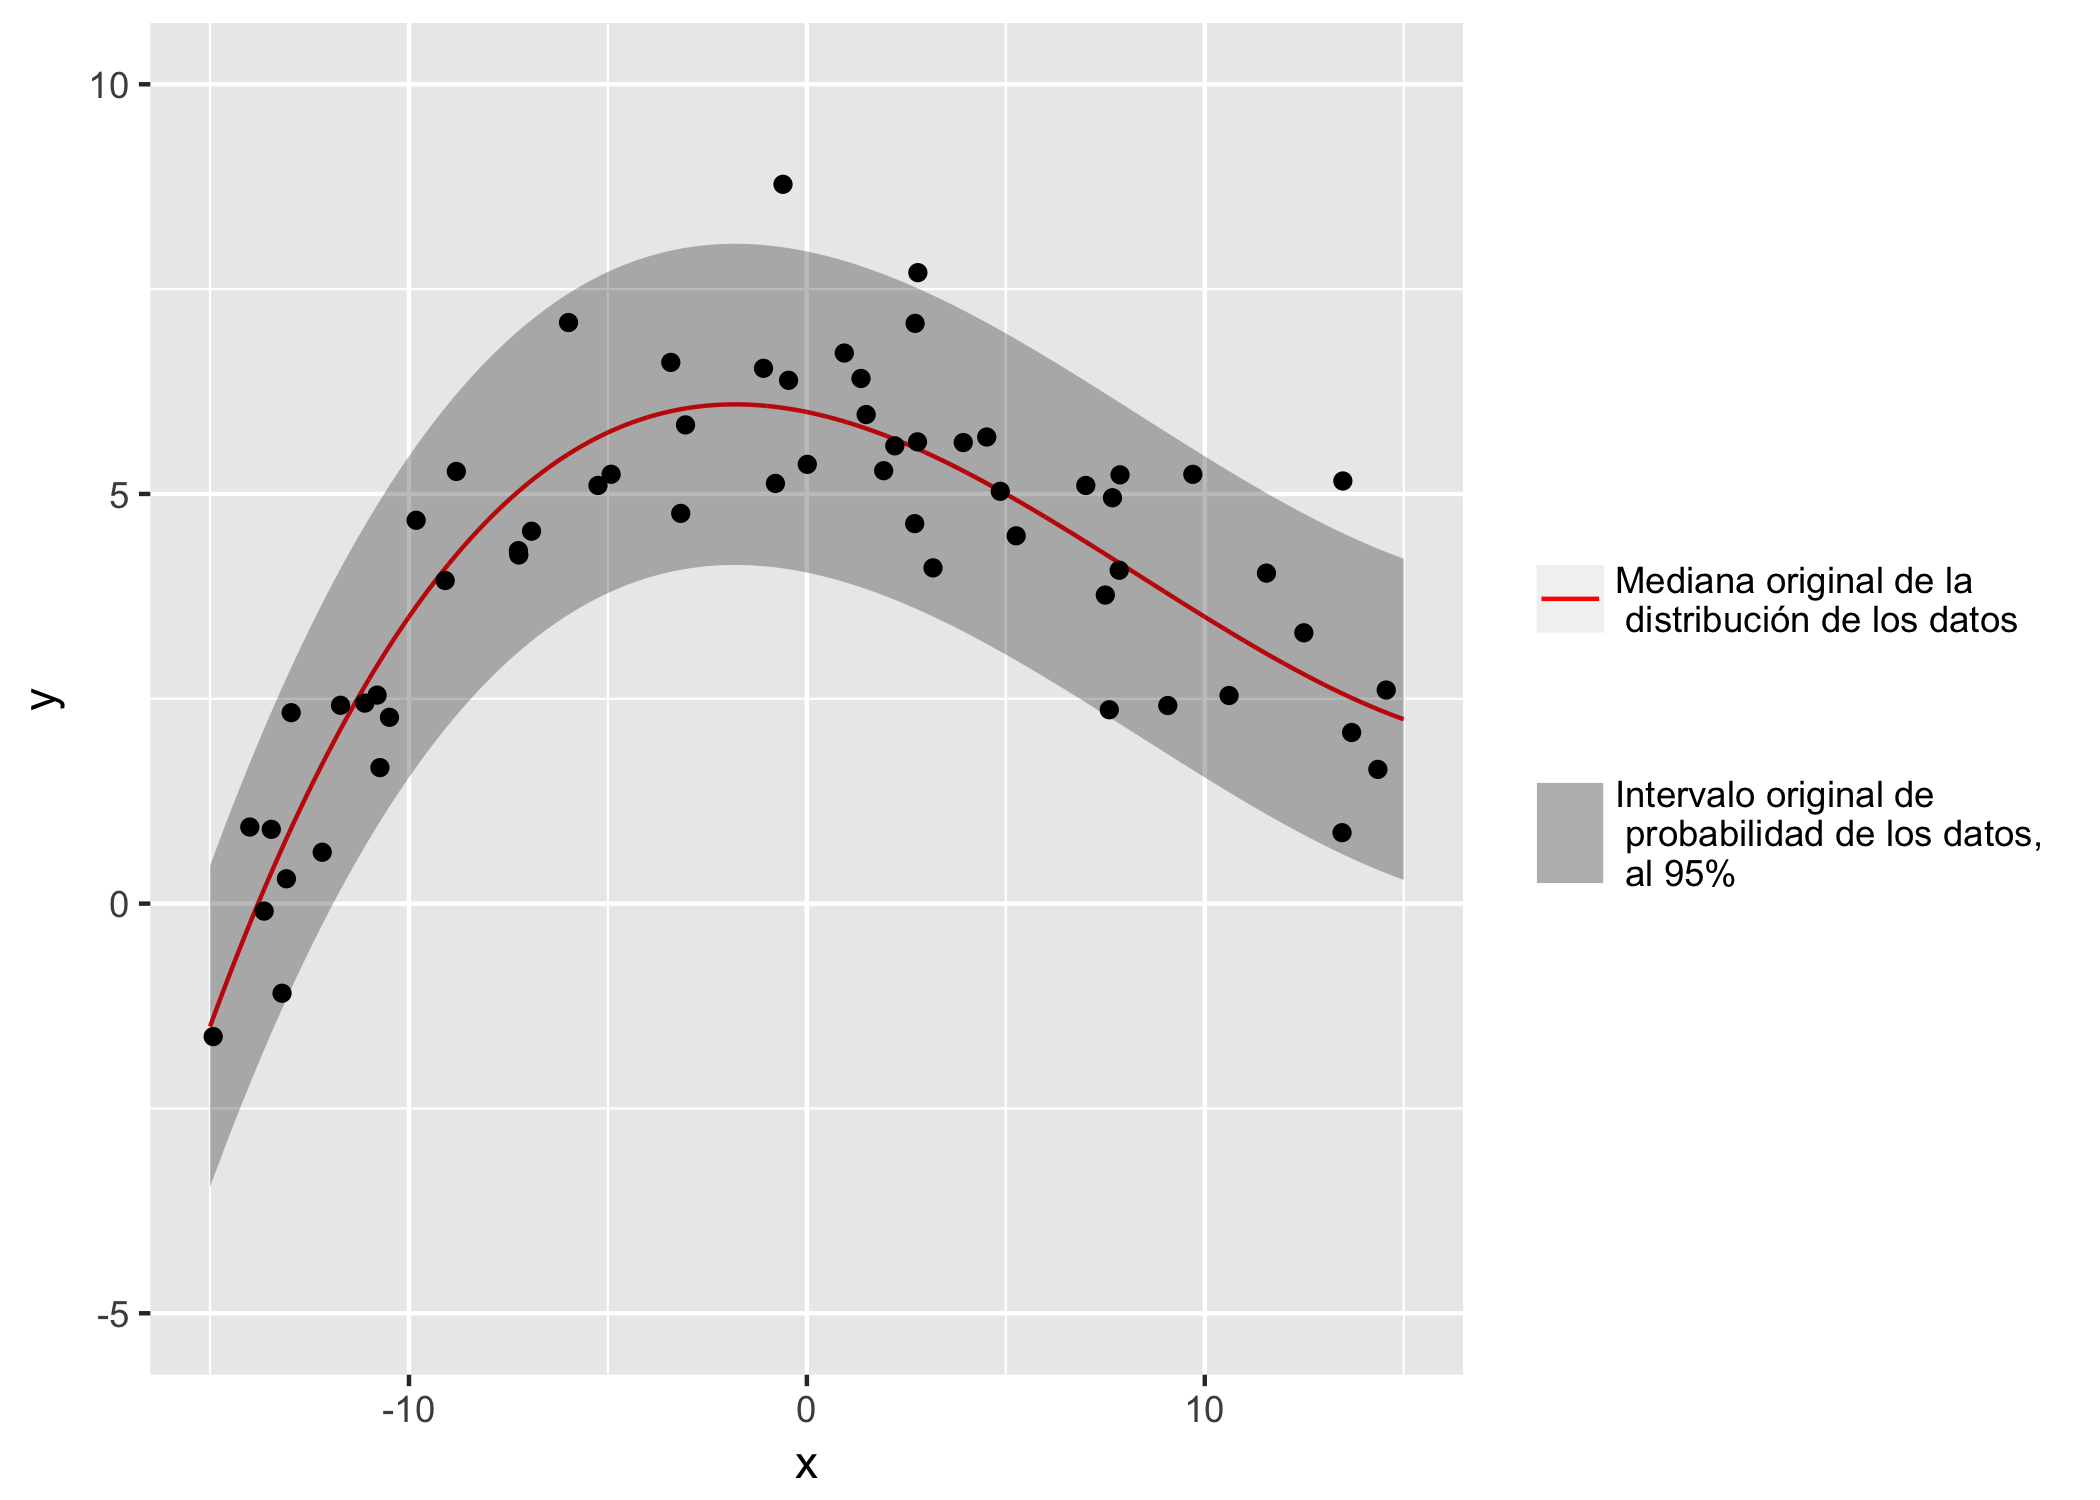
\includegraphics[width=0.7\textwidth]{Figures/Simulation/classic/sample.png}
	\label{sample_classic}
\end{figure}

Posteriormente se ajustaron los modelos y se realiz\'o predicci\'on de la forma en la que se explic\'o anteriormente, obteniendo los siguientes resultados.

\begin{table}[H]
\centering
\caption{Error cuadrático medio de datos que cumplen supuestos tradicionales de regresi\'on.} 
\begin{tabular}{ccc}
  \hline
Cuantil & Modelo Tradicional & Modelo GPDP \\ 
  \hline
0.95 & 0.84 & 0.83 \\ 
  0.50 & 0.02 & 0.19 \\ 
  0.25 & 0.23 & 0.16 \\ 
   \hline
\end{tabular}
\label{mse_classic}
\end{table}

\begin{table}[H]
\centering
\caption{Correlación al cuadrado de datos que cumplen supuestos tradicionales de regresi\'on.} 
\begin{tabular}{ccc}
  \hline
Cuantil & Modelo Tradicional & Modelo GPDP \\ 
  \hline
0.95 & 0.99 & 0.91 \\ 
  0.50 & 0.99 & 0.94 \\ 
  0.25 & 0.99 & 0.96 \\ 
   \hline
\end{tabular}
\label{corr_classic}
\end{table}

\begin{table}[H]
\centering
\caption{Porcentaje de valores reales dentro del intervalo de confianza de datos que cumplen supuestos tradicionales de regresi\'on.} 
\begin{tabular}{ccc}
  \hline
Cuantil & Modelo Tradicional & Modelo GPDP \\ 
  \hline
0.95 & 68\% & 96\% \\ 
  0.50 & 100\% & 100\% \\ 
  0.25 & 100\% & 100\% \\ 
   \hline
\end{tabular}
\label{within_classic}
\end{table}

\begin{figure}[htbp]
	\centering
	\caption{Ajuste de los modelos Tradicional y \textit{GPDP}, para un conjunto de datos que cumplen los supuestos tradicionales de regresi\'on.}
	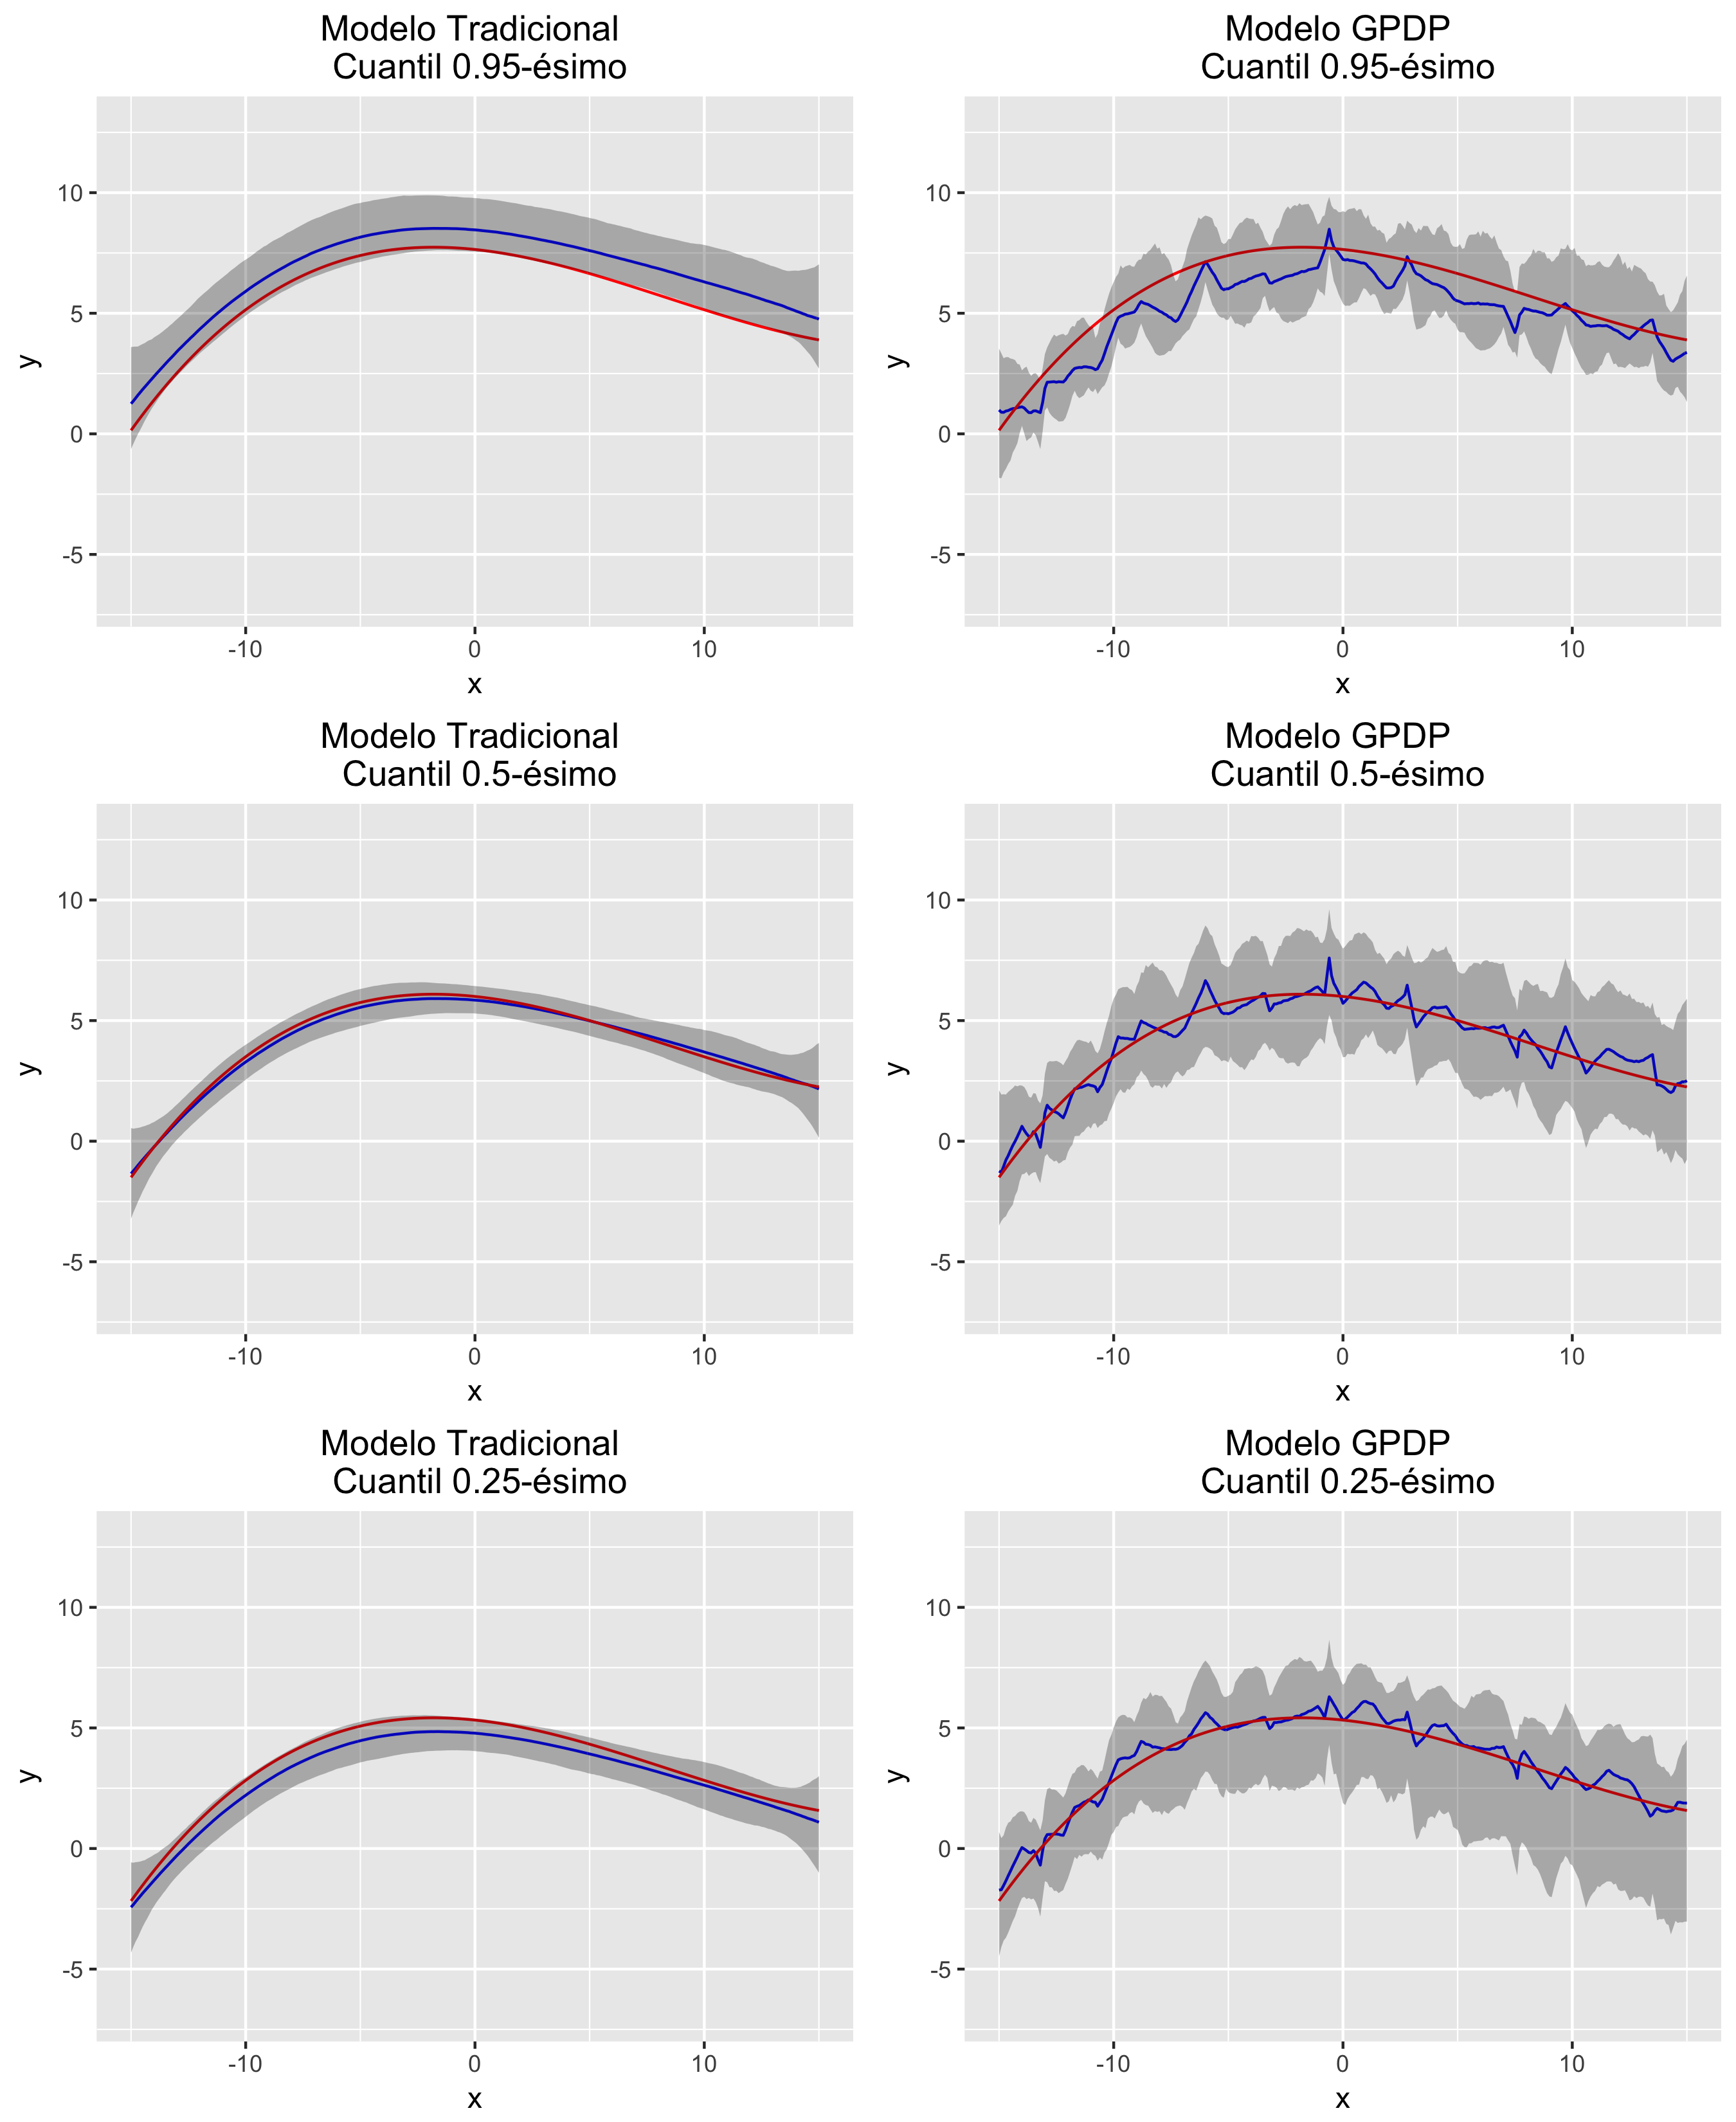
\includegraphics[width=\textwidth]{Figures/Simulation/classic/predictions.png}
	\captionsetup{singlelinecheck=off,font=footnotesize}
    \caption*{Nota: La l\'inea roja representa el valor real de cada cuantil, la l\'inea azul representa la mediana de la distribuci\'on posterior predictiva y el \'area gris su intervalo de probabilidad al 95\%.}
	\label{models_classic}
\end{figure}

Como era de esperarse, el modelo tradicional replic\'o de forma muy atinada el comportamiento polinomial de los datos. La m\'etrica que mejor refleja esta situaci\'on es la correlaci\'on al cuadrado, en donde dicho modelo obtuvo pr\'acticamente un valor perfecto para los tres cuantiles ajustados. Sin embargo, si bien no alcanz\'o los mismos niveles, el modelo GPDP tambi\'en obtuvo valores altos.

De hecho, si observa el cuadro \ref{mse_classic}, el lector podr\'a notar que para el cuantil $0.95$\textit{-\'esimo}, el error cuadr\'atico medio es pr\'acticamente el mismo, y para el cuantil $0.25$\textit{-\'esimo} es menor. Es decir, mientras que el modelo tradicional comprendi\'o de mejor manera las subidas y bajadas puntuales de la funci\'on, el modelo GPDP fue m\'as certero para estimar el nivel, conforme los valores se alejaron de la mediana. 

Lo anterior es confirmado por la tabla \ref{within_classic}, ya que para el caso del ajuste tradicional del cuantil $0.95$\textit{-\'esimo} \'unicamente el $68\%$ de los valores reales del cuantil quedaron dentro del angosto intervalo de probabilidad. Mi hip\'otesis es que dicho error de estimaci\'on del nivel proviene de un error min\'usculo de ajuste de la distribuci\'on de $\sigma^2$, el cual queda totalmente desapercibido en la estimaci\'on casi perfecta de la mediana, pero en un valor extremo, como es el caso del cuantil $0.95$\textit{-\'esimo}, s\'i se ve reflejado.

Hay comentarios del ajuste de este conjunto de datos que coincidir\'an con otros, por lo que en la secci\'on \ref{models_comp} se har\'an apuntes generales acerca de ellos.

Por otro lado, como se detall\'o en el cap\'itulo anterior, con el uso del paquete \textit{GPDPQuantReg} tambi\'en es posible obtener diagn\'osticos de las cadenas de Markov del modelo GPDP, los cuales se explican de manera m\'as detallada en el \autoref{chap:MCMC}. Como ejemplo, se presentan los del ajuste del cu\'antil $0.5$-\textit{\'esimo} para los datos de esta subsecci\'on, en la figura \ref{diag_sgse}. Los par\'ametros que se analizan son la $\lambda$, par\'ametro de escala de la funci\'on covarianza del proceso Gaussiano; y, adem\'as, se eligi\'o una observaci\'on de forma aleatoria, para la que se dio seguimiento al valor de $\sigma$ y $f_p(x)$. 

\begin{figure}[H]
	\centering
	\caption{Diagn\'osticos de las cadenas de Markov del cu\'antil $0.5$-\textit{\'esimo}, de datos que cumplen los supuestos tradicionales de regresi\'on.}
	\subfloat[Ergodicidad]{
	    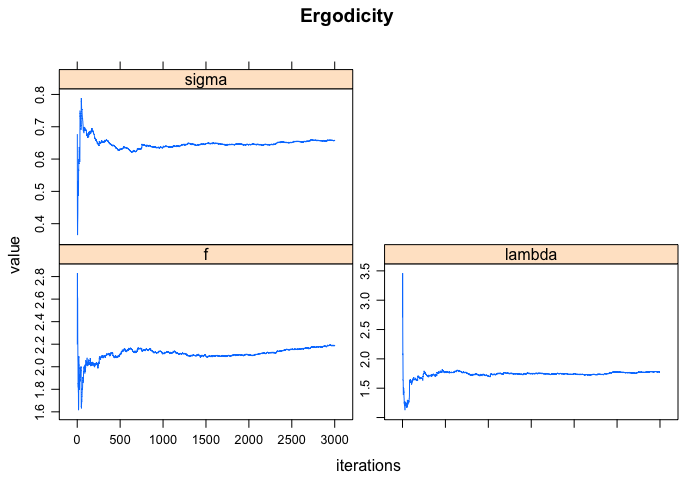
\includegraphics[width=0.45\textwidth]{Figures/Simulation/classic/diagnostics/ergodicity.png}
	}
	\subfloat[Autocorrelaci\'on]{
	    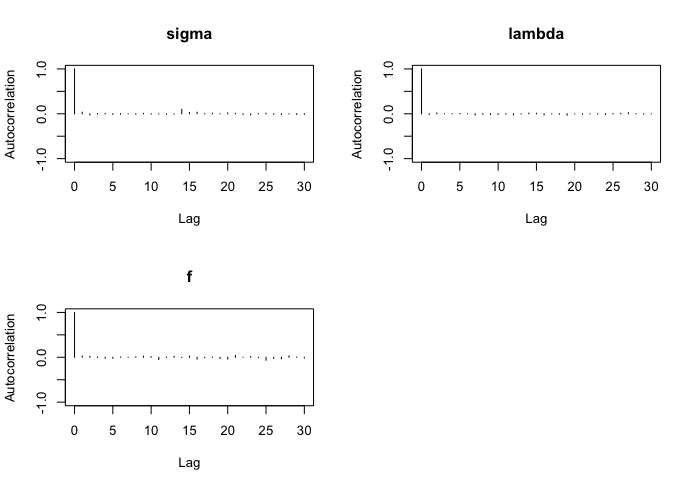
\includegraphics[width=0.45\textwidth]{Figures/Simulation/classic/diagnostics/autocorrelation.png}
	}\\
	\subfloat[Correlaci\'on cruzada]{
	    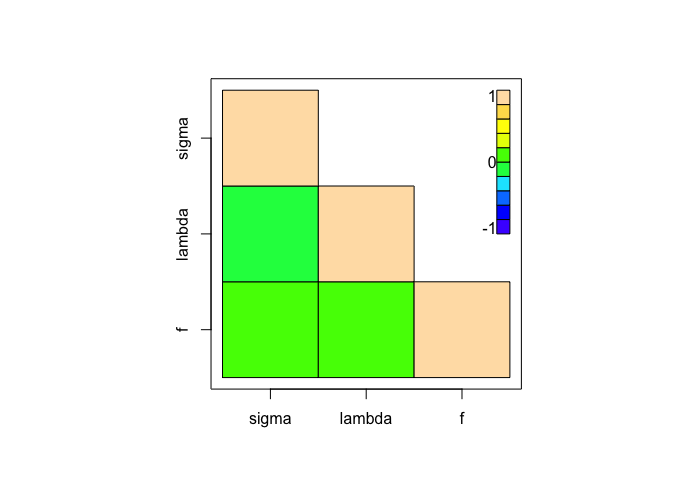
\includegraphics[width=0.45\textwidth]{Figures/Simulation/classic/diagnostics/crosscorrelation.png}
	}
	\subfloat[Traza]{
	    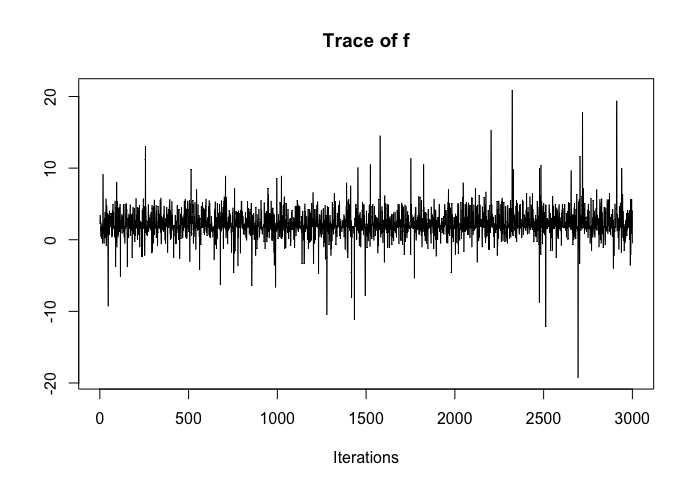
\includegraphics[width=0.45\textwidth]{Figures/Simulation/classic/diagnostics/trace.png}
	}
	\label{diag_sgse}
\end{figure}

La ergodicidad parece adecuada, debido a que después de las primeras iteraciones, el promedio del valor de los par\'ametros se estabiliza en un nivel relativamente fijo para todas las iteraciones siguientes. La autocorrelaci\'on es excelente, ya que para los tres par\'ametros validados se muestra el valor de 1 en la correlaci\'on consigo mismo (por construcci\'on, siempre es as\'i), pero a partir del siguiente valor en la cadena de Markov, la correlaci\'on es pr\'acticamente 0. Es decir, los valores simulados s\'i parecen haber sido simulados de la distribuci\'on posterior, de forma independiente entre s\'i.

La correlaci\'on cruzada entre par\'ametros tambi\'en es cercana a 0, por lo que la simulaci\'on de un par\'ametro de la cadena no muestra una gran dependencia del valor de otro par\'ametro, en la misma iteraci\'on. Por ello, hay motivos para pensar que la cadena de Markov no cay\'o en ciclos distintos a su distribuci\'on estacionaria. De hecho, esto se puede confirmar al observar la traza de $f$, ya que no muestra comportamientos c\'iclicos y aunque se centra en cierto intervalo de valores, tambi\'en hay simulaciones que salen de \'el de forma espor\'adica.

\subsection{Error de colas pesadas}

En el siguiente conjunto de datos se utiliz\'o la distribuci\'on Cauchy para simular el error. A pesar de ser sim\'etrica y centrada en 0, dicha distribuci\'on es peculiar debido a que su esperanza y varianza no est\'an definidas. El motivo de ello son sus colas pesadas, mismas que originan con cierta frecuencia valores muy alejados del centro. Adem\'as, se introdujo un componente sinoidal en la funci\'on tendencia, mismo que puede ser aproximado con un polinomio tanto como se quiera, utilizando t\'erminos de su serie de Taylor. Sin embargo, tambi\'en tiene un valor absoluto, que requiere un n\'umero grande de t\'erminos para poder ser aproximado certeramente por la familia de los polinomios.

La expresi\'on de la funci\'on tendencia utilizada es \begin{equation*}
    g(x) = \frac{1}{4}|x| + sen(x).
\end{equation*}
Por otro lado, el error se distribuy\'o $\omega(x) \sim Cauchy(0,0.1)$. Los datos obtenidos se pueden observar en la figura \ref{sample_heavy_tails}.

\begin{figure}[H]
	\centering
	\caption{Datos simulados con error de colas pesadas.}
	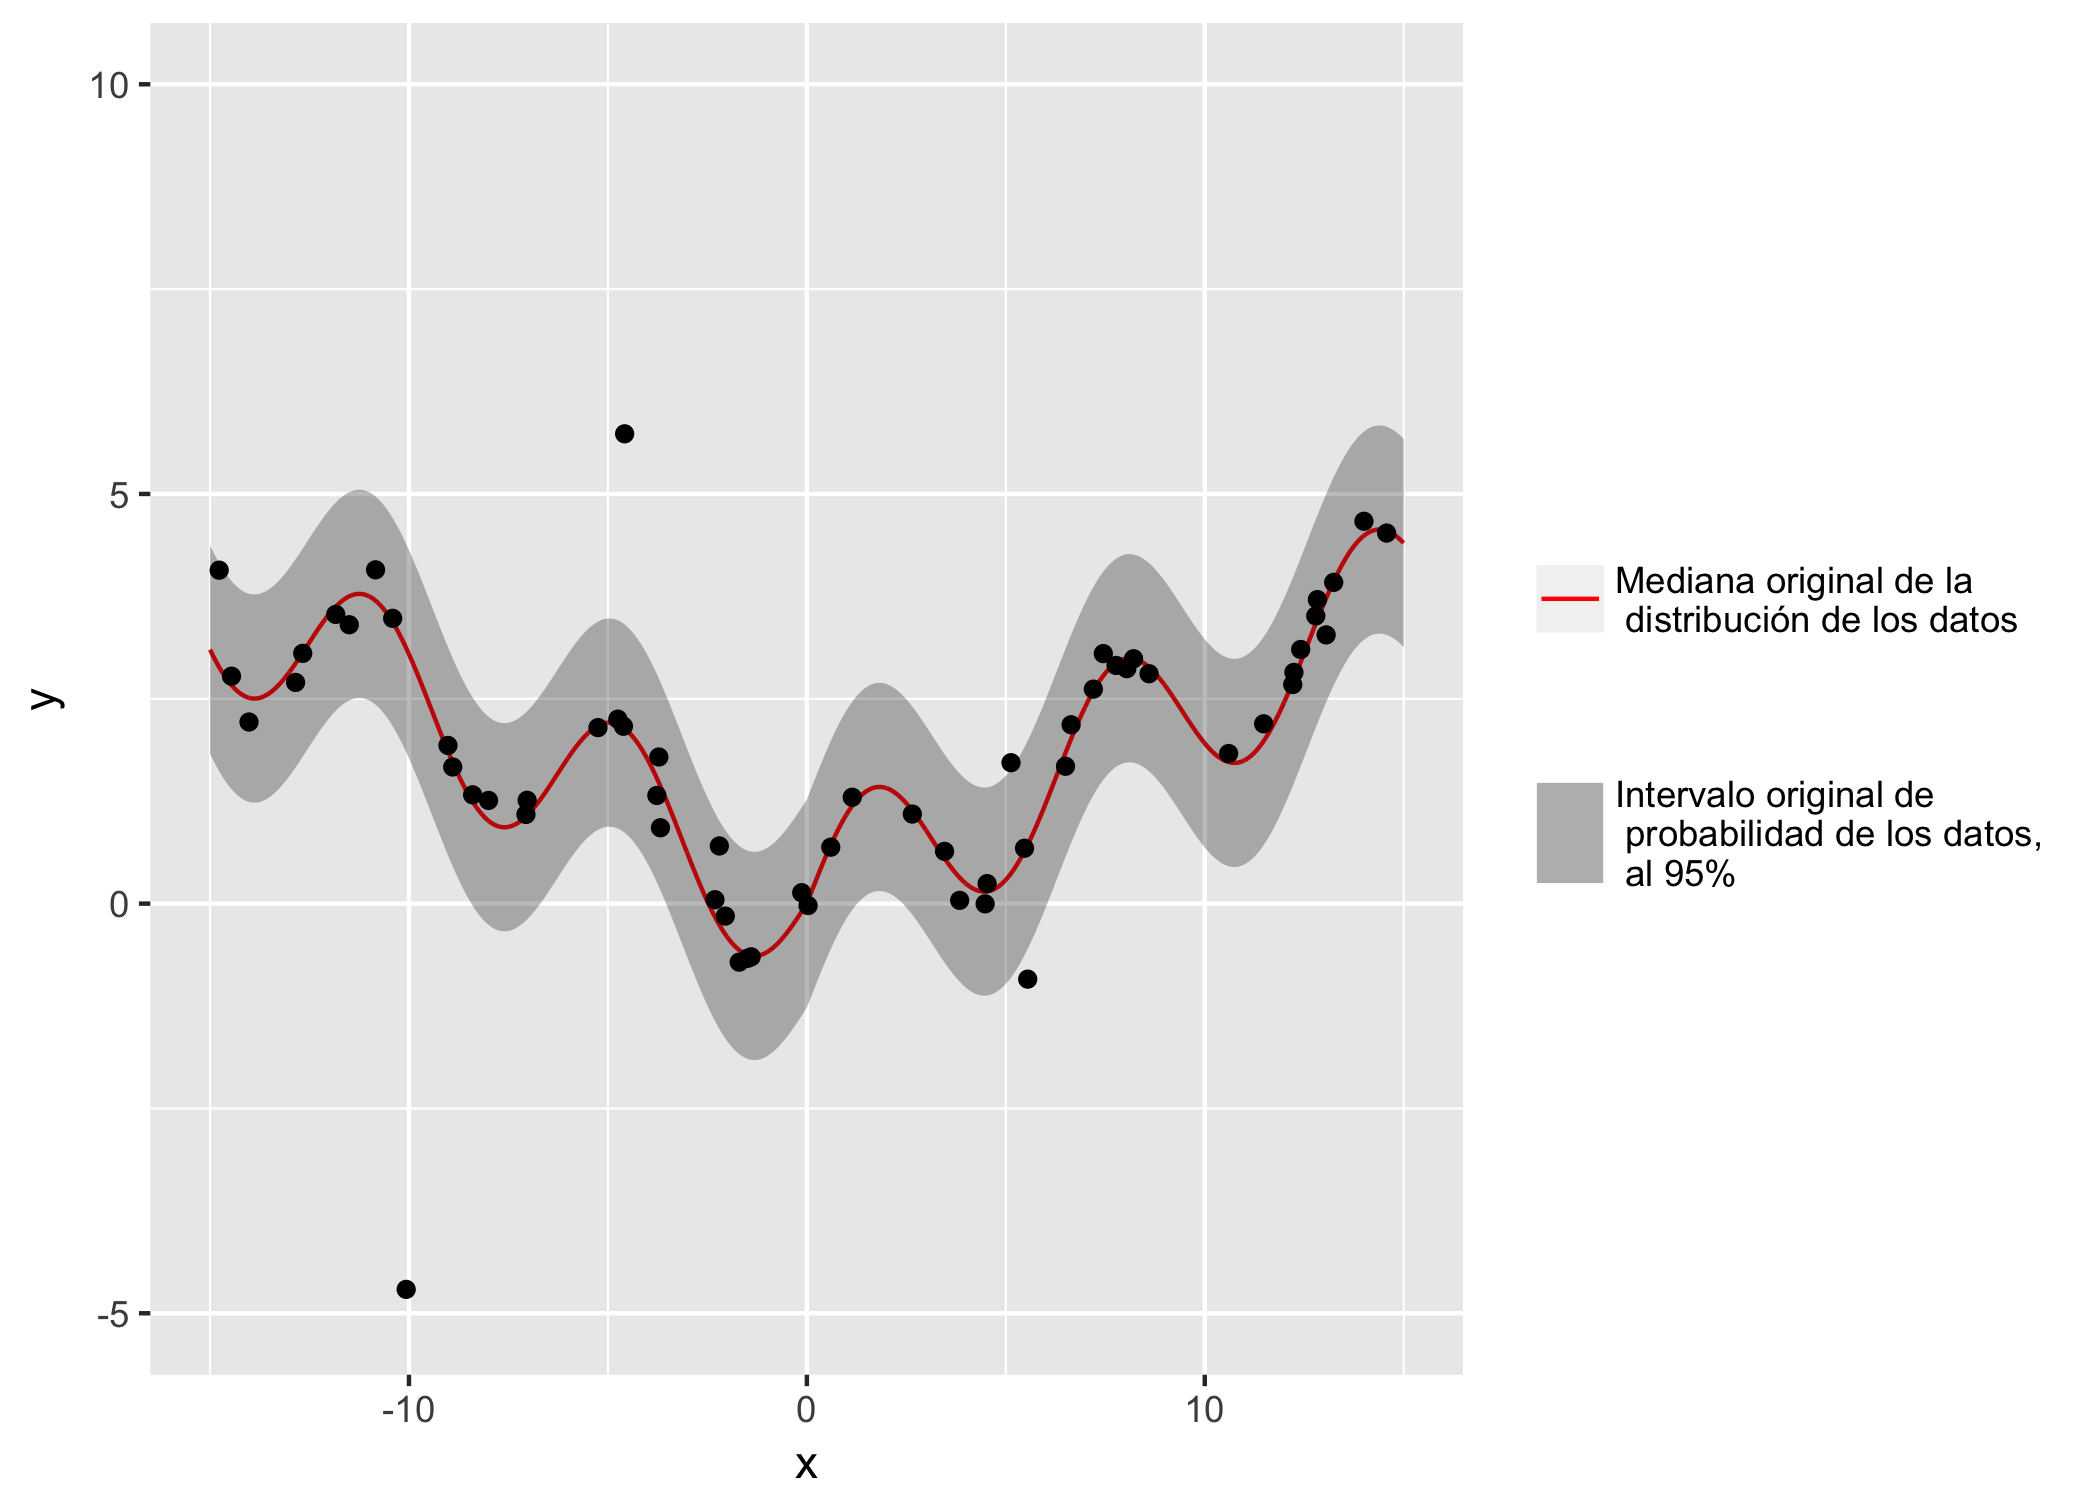
\includegraphics[width=0.7\textwidth]{Figures/Simulation/heavy_tails/sample.png}
	\label{sample_heavy_tails}
\end{figure}

Como se puede observar, la mayor\'ia de los datos est\'an concentrados alrededor de la funci\'on tendencia. Sin embargo, ocasionalmente los valores se disparan y se alejan ampliamente de dicha concentraci\'on. Claros ejemplos son el dato que est\'a muy por debajo de los dem\'as, cerca de $x = -10$, y uno que est\'a muy por arriba, alrededor de $x = -5$. Lo interesante de este ejemplo fue ver c\'omo se comportaban ambos modelos ante dichos datos at\'ipicos. Los resultados se muestran a continuaci\'on.

\begin{table}[H]
\centering
\caption{Error cuadrático medio de datos con error de colas pesadas.} 
\begin{tabular}{ccc}
  \hline
Cuantil & Modelo Tradicional & Modelo GPDP \\ 
  \hline
0.95 & 5.42 & 0.18 \\ 
  0.50 & 0.61 & 0.75 \\ 
  0.25 & 1.89 & 1.12 \\ 
   \hline
\end{tabular}
\label{mse_heavy_tails}
\end{table}

\begin{table}[H]
\centering
\caption{Correlación al cuadrado de datos con error de colas pesadas.} 
\begin{tabular}{ccc}
  \hline
Cuantil & Modelo Tradicional & Modelo GPDP \\ 
  \hline
0.95 & 0.64 & 0.91 \\ 
  0.50 & 0.64 & 0.64 \\ 
  0.25 & 0.64 & 0.57 \\ 
   \hline
\end{tabular}
\label{corr_heavy_tails}
\end{table}

\begin{table}[H]
\centering
\caption{Porcentaje de valores reales dentro del intervalo de confianza de datos con error de colas pesadas.} 
\begin{tabular}{ccc}
  \hline
Cuantil & Modelo Tradicional & Modelo GPDP \\ 
  \hline
0.95 & 9\% & 98\% \\ 
  0.50 & 57\% & 100\% \\ 
  0.25 & 41\% & 96\% \\ 
   \hline
\end{tabular}
\label{within_heavy_tails}
\end{table}

\begin{figure}[htbp]
	\centering
	\caption{Ajuste de los modelos Tradicional y \textit{GPDP}, para un conjunto de datos con error de colas pesadas.}
	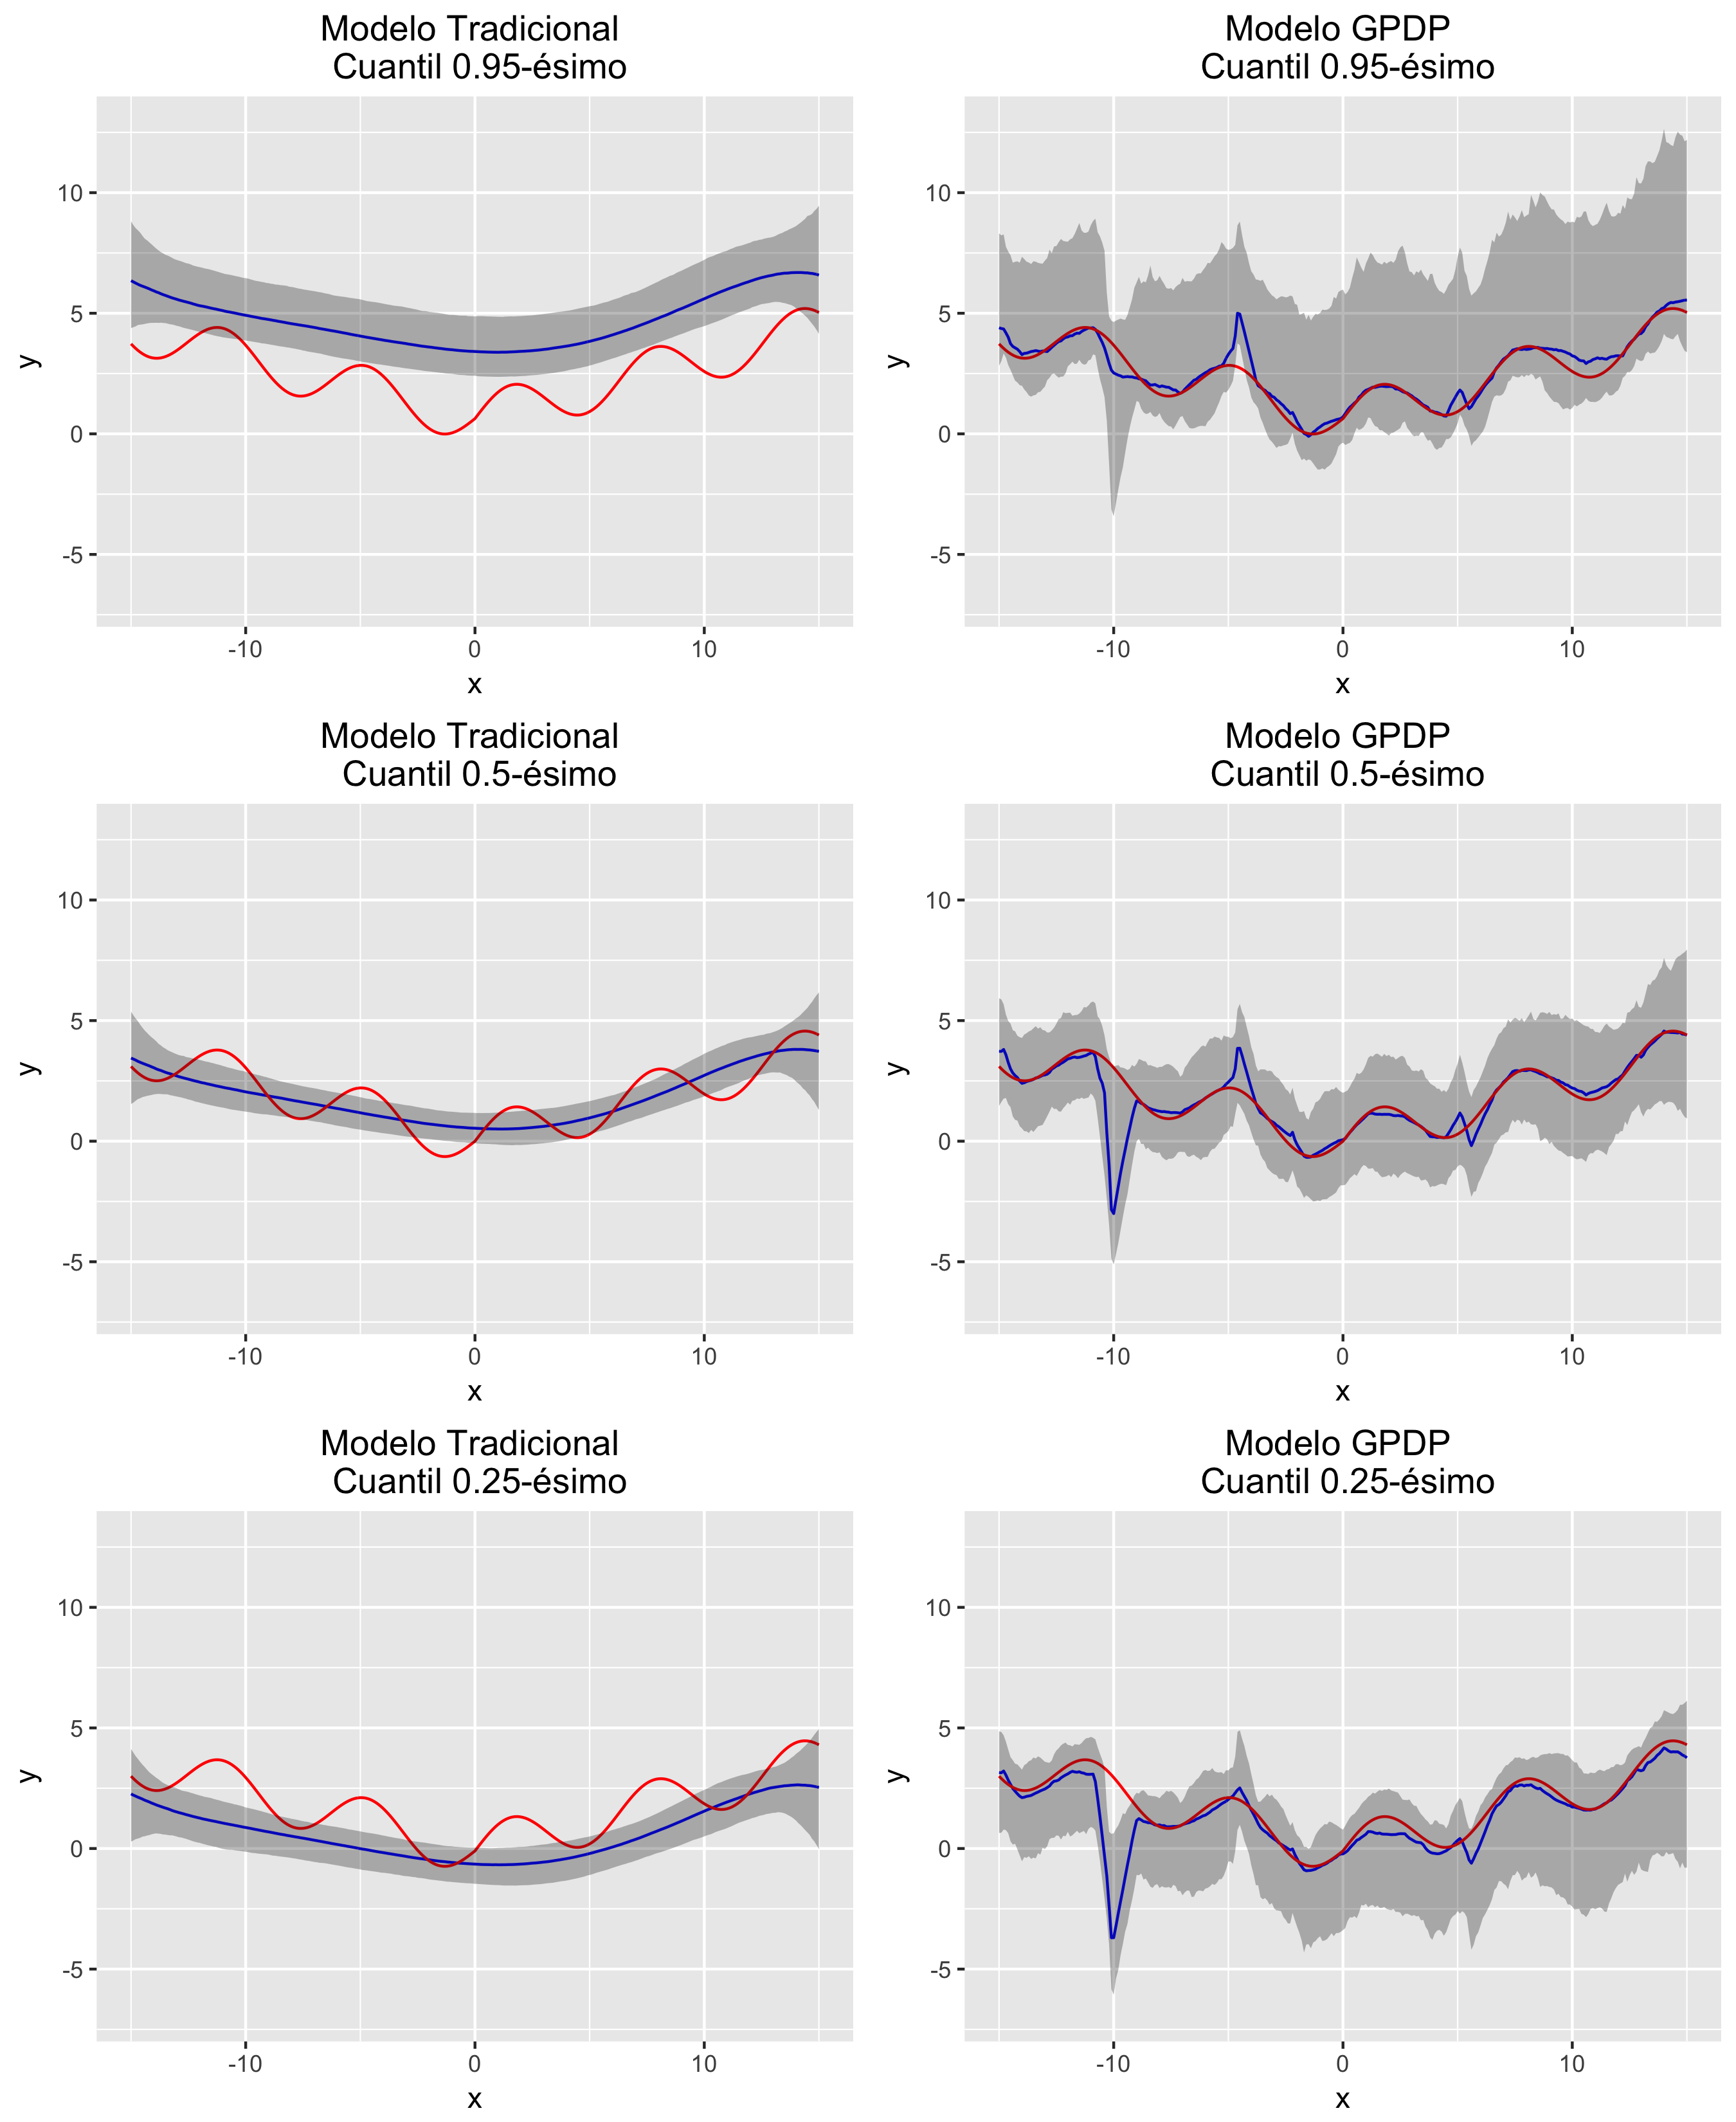
\includegraphics[width=\textwidth]{Figures/Simulation/heavy_tails/predictions.png}
	\captionsetup{singlelinecheck=off,font=footnotesize}
    \caption*{Nota: La l\'inea roja representa el valor real de cada cuantil, la l\'inea azul representa la mediana de la distribuci\'on posterior predictiva y el \'area gris su intervalo de probabilidad al 95\%.}
	\label{models_heavy_tails}
\end{figure}

Una vez obtenidos los resultados de ambos modelos, resulta interesante observar varios aspectos de la figura \ref{models_heavy_tails}. Tocando el tema de la influencia de valores at\'ipicos, parece claro que el modelo tradicional los manej\'o estimando valores muy altos para $\sigma^2$, del error que supone normal. Esto ocasion\'o que para los cuantiles distintos a la mediana, estimara que estaban m\'as lejos del centro, de lo que realmente estaban. Dicha situaci\'on se puede confirmar utilizando el cuadro \ref{within_heavy_tails}, ya que s\'olo el $41\%$ de los datos reales cay\'o dentro del intervalo de probabilidad estimado para el cuantil $0.25$\textit{-\'esimo}, y peor a\'un para el $0.95$\textit{-\'esimo}, donde s\'olo el $9\%$ lo hizo.

En cuanto a la estimaci\'on de la tendencia, el modelo tradicional interpret\'o que los datos ven\'ian de lo que parece ser una par\'abola, con m\'inimo y centro en 0, acerc\'andose relativamente al comportamiento del valor absoluto. Desafortunadamente no logr\'o atrapar el comportamiento sinoidal y atribuy\'o las fluctuaciones al error aleatorio. Eso se puede ver claramente en su estimaci\'on del cuantil $0.5$\textit{-\'esimo}, donde captur\'o el nivel de manera adecuada, pero como muestra la figura \ref{models_heavy_tails} y el cuadro \ref{corr_heavy_tails}, muchos valores salieron tanto por arriba, como por abajo, del intervalo.

Por otro lado, el modelo GPDP hizo una estimaci\'on muy certera en la mayor\'ia de los puntos, como se refleja en los cuadros \ref{mse_heavy_tails} y \ref{within_heavy_tails}. La vecindad alrededor de $x = 10$, que coincide con el valor at\'ipico m\'as dram\'atico, es donde el ajuste pudo haber sido mucho mejor. Sin embargo, creo que es importante recalcar que el problema se limit\'o a un error de estimaci\'on local, que no afect\'o a los puntos m\'as alla de cierta pequeña vecindad. De hecho, el siguiente valor at\'ipico en magnitud, alrededor de $x = 5$, fue manejado aceptablemente por el modelo para los tres cuantiles.

\subsection{Heterocedasticidad}

Otro supuesto com\'un en muchos modelos de regresi\'on es la homocedasticidad, es decir, que los errores no dependen de $x$. Para este ejemplo particular decid\'i observar c\'omo afectar\'ia a la estimaci\'on el hecho de que la distribuci\'on de los errores aleatorios dependiera del valor de la variable explicativa, es decir, datos que presentaran heterocedasticidad.

Para ello se us\'o como funci\'on de tendencia al polinomio de primer orden 
\begin{equation*}
    g(x) = \frac{1}{10}x + 2,
\end{equation*}
y la complejidad de estimaci\'on recay\'o en el error $\omega(x) \sim \mathcal{N}\left(0,\frac{|x|}{10}\right)$. 

\begin{figure}[H]
	\centering
	\caption{Datos simulados con heterocedasticidad.}
	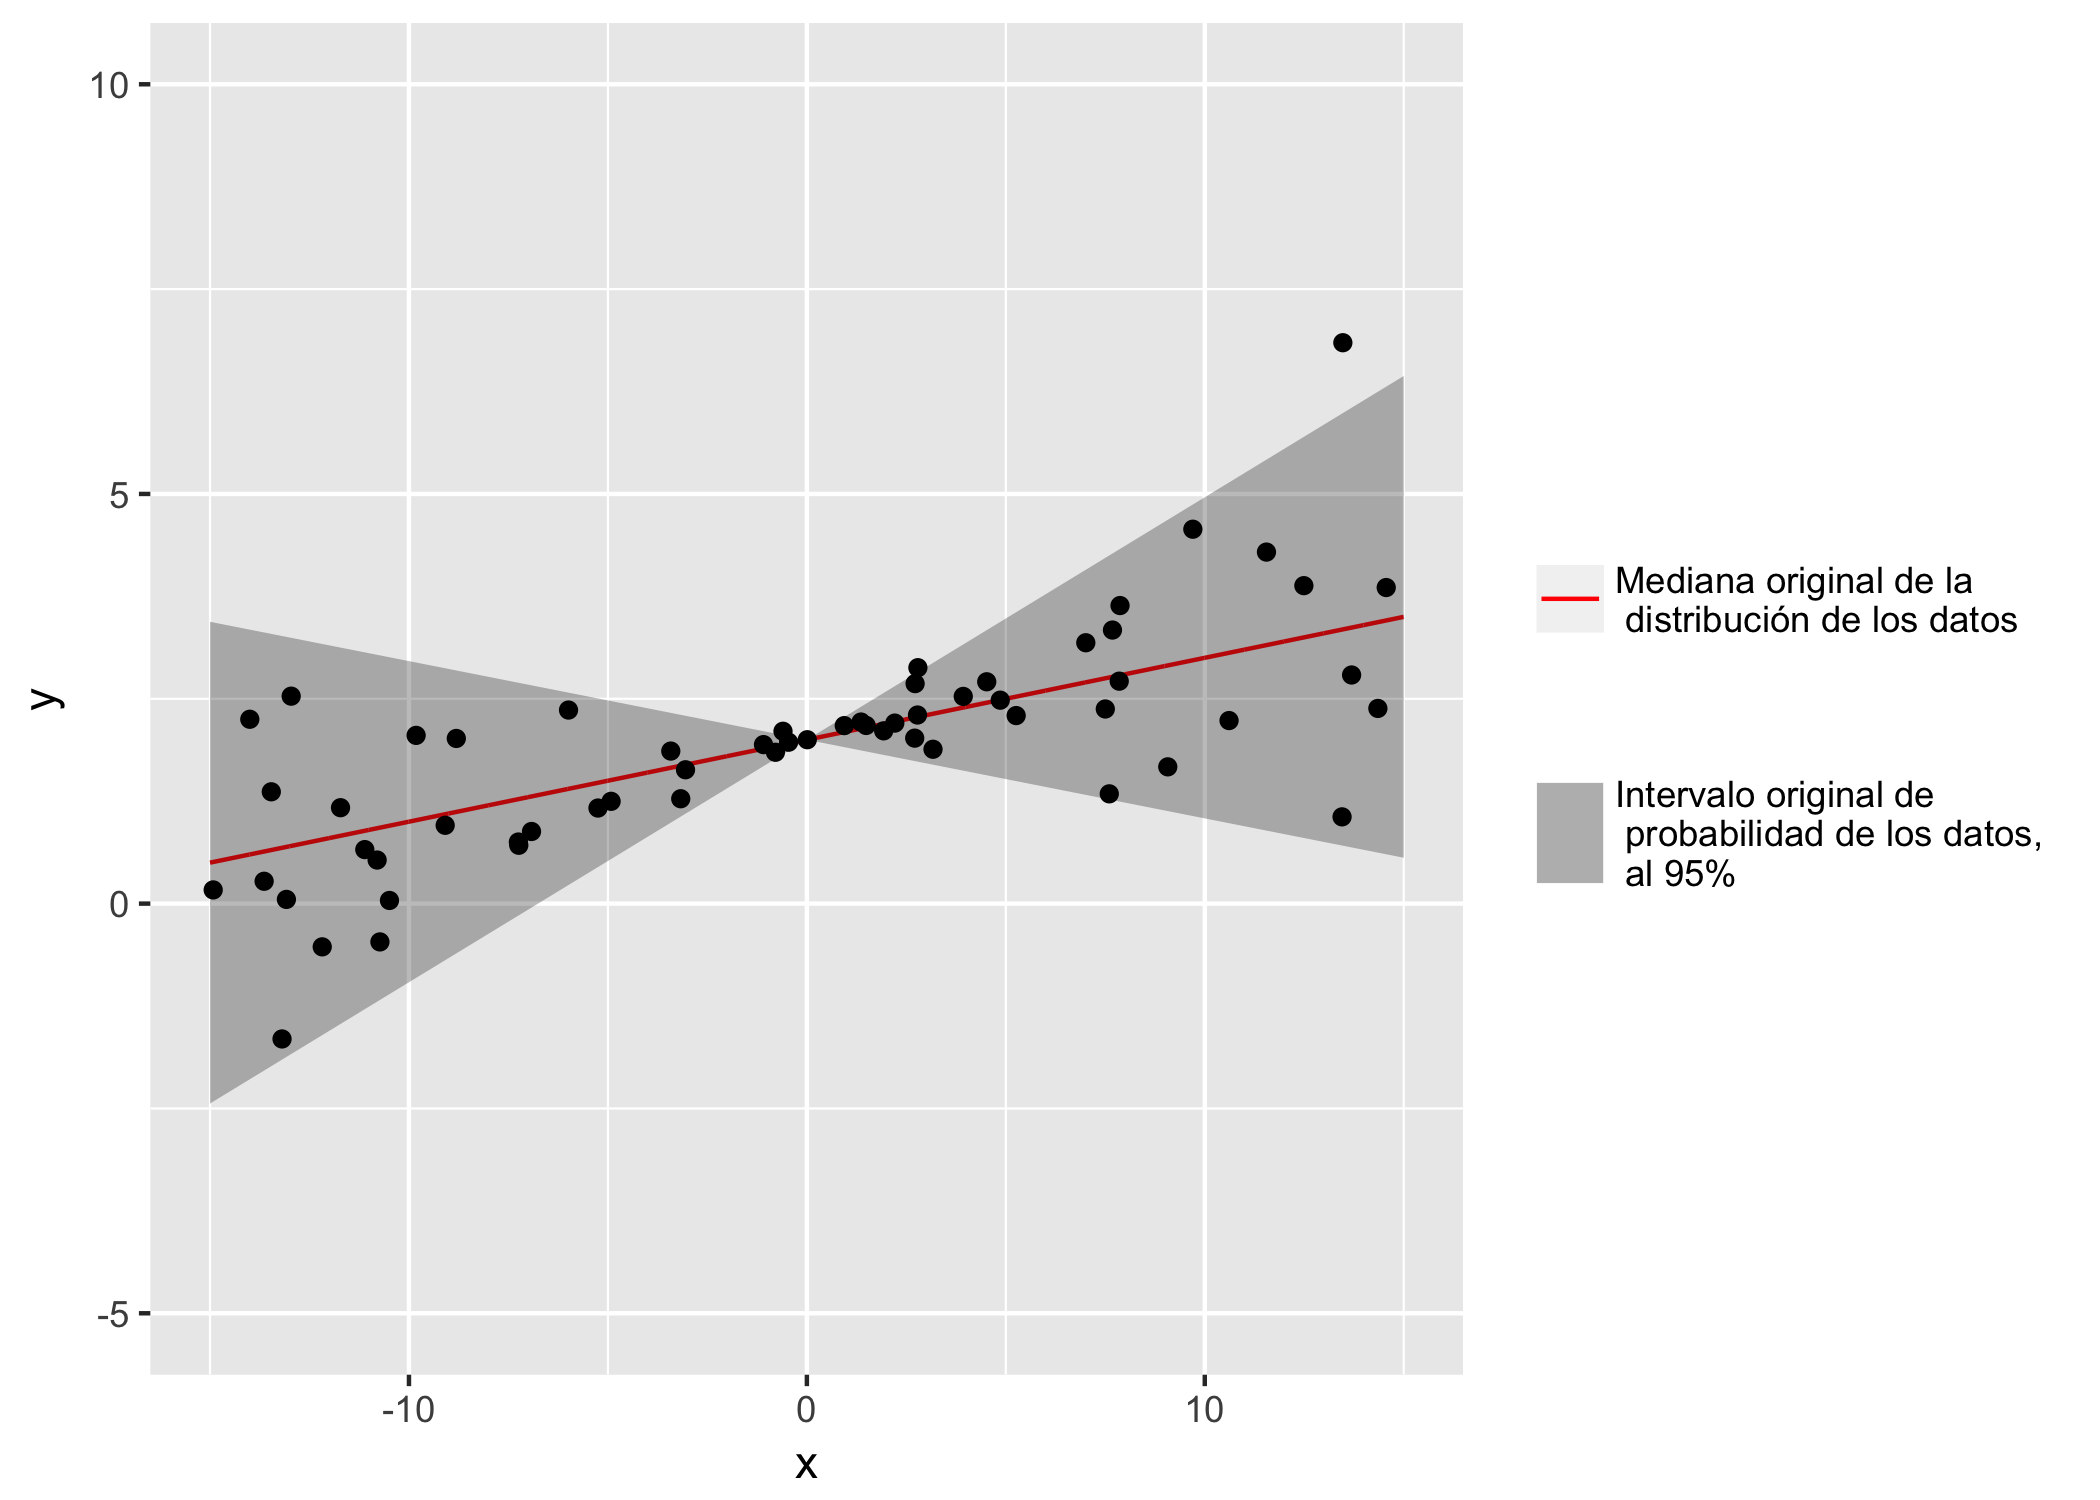
\includegraphics[width=0.7\textwidth]{Figures/Simulation/heteroscedasticity/sample.png}
	\label{sample_heteroscedasticity}
\end{figure}

Como se puede observar en la figura \ref{sample_heteroscedasticity}, \'unicamente la mediana de los datos es una l\'inea totalmente recta. Los dem\'as cuantiles se expresan como dos rectas con distinta pendiente, que se unen en el punto $x = 0$. Este comportamiento, similar al valor absoluto, tampoco se puede expresar fielmente con polinomios, sino que s\'olo se puede aproximar. A continuaci\'on se presentan los resultados del ajuste de ambos modelos.

\begin{table}[H]
\centering
\caption{Error cuadrático medio de datos que presentan heterocedasticidad.} 
\begin{tabular}{ccc}
  \hline
Cuantil & Modelo Tradicional & Modelo GPDP \\ 
  \hline
0.95 & 0.51 & 0.58 \\ 
  0.50 & 0.02 & 0.17 \\ 
  0.25 & 0.15 & 0.14 \\ 
   \hline
\end{tabular}
\label{mse_heteroscedasticity}
\end{table}

\begin{table}[H]
\centering
\caption{Correlación al cuadrado de datos que presentan heterocedasticidad.} 
\begin{tabular}{ccc}
  \hline
Cuantil & Modelo Tradicional & Modelo GPDP \\ 
  \hline
0.95 & 0.63 & 0.78 \\ 
  0.50 & 0.98 & 0.86 \\ 
  0.25 & 0.86 & 0.84 \\ 
   \hline
\end{tabular}
\label{corr_heteroscedasticity}
\end{table}

\begin{table}[H]
\centering
\caption{Porcentaje de valores reales dentro del intervalo de confianza de datos que presentan heterocedasticidad.} 
\begin{tabular}{ccc}
  \hline
Cuantil & Modelo Tradicional & Modelo GPDP \\ 
  \hline
0.95 & 68\% & 95\% \\ 
  0.50 & 100\% & 100\% \\ 
  0.25 & 81\% & 100\% \\ 
   \hline
\end{tabular}
\label{within_heteroscedasticity}
\end{table}

\begin{figure}[htbp]
	\centering
	\caption{Ajuste de los modelos Tradicional y \textit{GPDP}, para un conjunto de datos con heterocedasticidad.}
	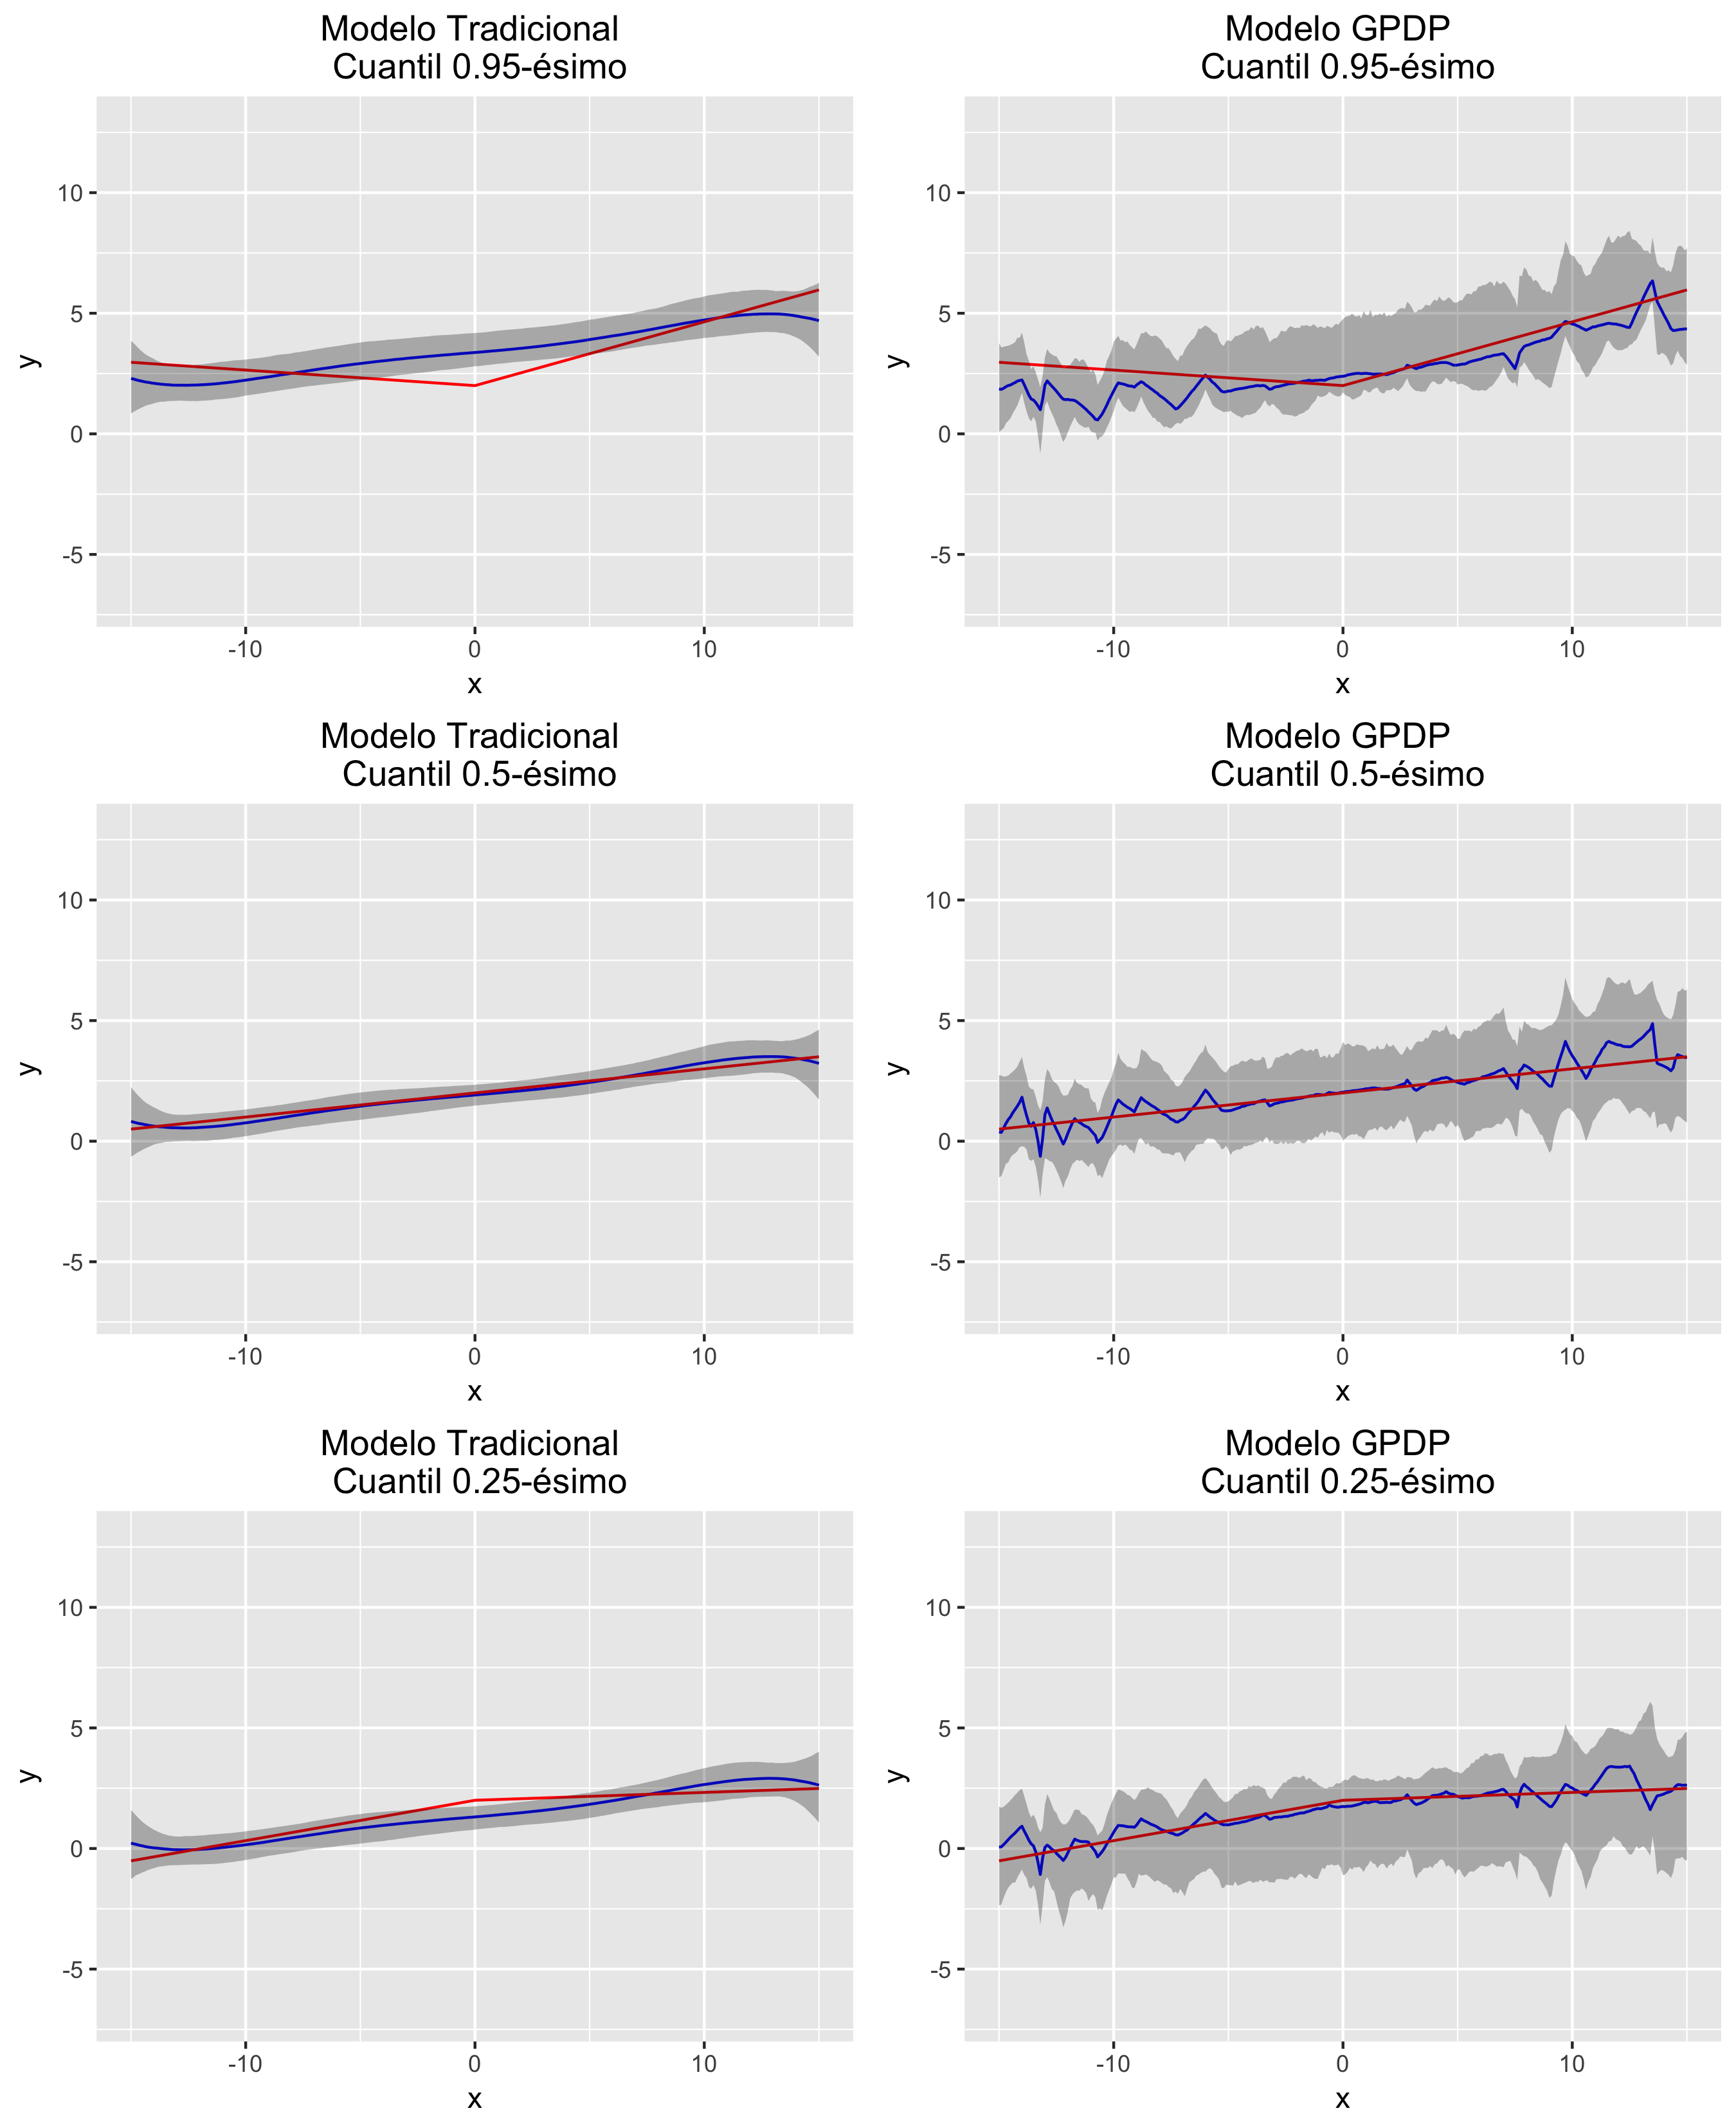
\includegraphics[width=\textwidth]{Figures/Simulation/heteroscedasticity/predictions.png}
	\captionsetup{singlelinecheck=off,font=footnotesize}
    \caption*{Nota: La l\'inea roja representa el valor real de cada cuantil, la l\'inea azul representa la mediana de la distribuci\'on posterior predictiva y el \'area gris su intervalo de probabilidad al 95\%.}
	\label{models_heteroscedasticity}
\end{figure}

Como se puede observar en la figura \ref{models_heteroscedasticity}, el modelo tradicional interpret\'o el valor de todos los cuantiles como una simple l\'inea recta, \'unicamente variando la ordenada al origen. De hecho, el modelo de la mediana logr\'o una estimaci\'on excelente, como lo reafirman los cuadros \ref{mse_heteroscedasticity}, \ref{corr_heteroscedasticity} y \ref{within_heteroscedasticity}. Sin embargo, conforme la estimaci\'on se fue alejando de la mediana y los valores reales de los cuantiles fueron distingui\'endose de la l\'inea recta, la calidad de la estimaci\'on predictiva se redujo dr\'asticamente.

En cuanto al modelo GPDP, los cuadros \ref{mse_heteroscedasticity}, \ref{corr_heteroscedasticity} y \ref{within_heteroscedasticity} tambi\'en muestran que conforme se tom\'o un cuantil m\'as lejano a la mediana, la calidad de la estimaci\'on empeor\'o. Sin embargo, la ca\'ida fue menos fuerte, particularmente para las medidas de correlaci\'on y porcentaje de valores dentro del intervalo. Esto se debe principalmente a que el modelo tradicional modela la media, y a partir de ah\'i cada cuantil s\'olo representa un cambio de nivel, pero manteniendo la forma de la funci\'on. En cambio, el modelo GPDP contempla que cada cuantil puede tener una forma propia, distinta de los otros cuantiles.

\subsection{Error asim\'etrico}

Hasta este punto se han realizado perturbaciones al modelo tradicional de regresi\'on en la forma de la distribuci\'on de los datos (colas pesadas y heterocedasticidad). Sin embargo, dichas perturbaciones mantuvieron una caracter\'istica del modelo tradicional: la simetr\'ia del error. En el siguiente conjunto de datos se desafi\'o dicha condici\'on, usando un error aleatorio asim\'etrico. Particularmente se utiliz\'o $\omega(x) \sim Gamma(1,1)$.

La funci\'on tendencia involucr\'o a las funciones coseno y exponencial, ambas pudi\'endose aproximar de buena forma con polinomios, utilizando sus series de Taylor. Sin embargo, cabe recordar que \'unicamente se est\'an utilizando polinomios de grado 5 en el modelo tradicional, por lo que podr\'ian resultar insuficientes. Su expresi\'on matem\'atica fue
\begin{equation*}
    g(x) = \frac{1}{5} x cos(x) - \frac{1}{5}exp\left(\frac{x}{10}\right).
\end{equation*}
Los datos obtenidos despu\'es de simular se pueden observar en la figura \ref{sample_asymmetric}.

\begin{figure}[H]
	\centering
	\caption{Datos simulados con error asim\'etrico.}
	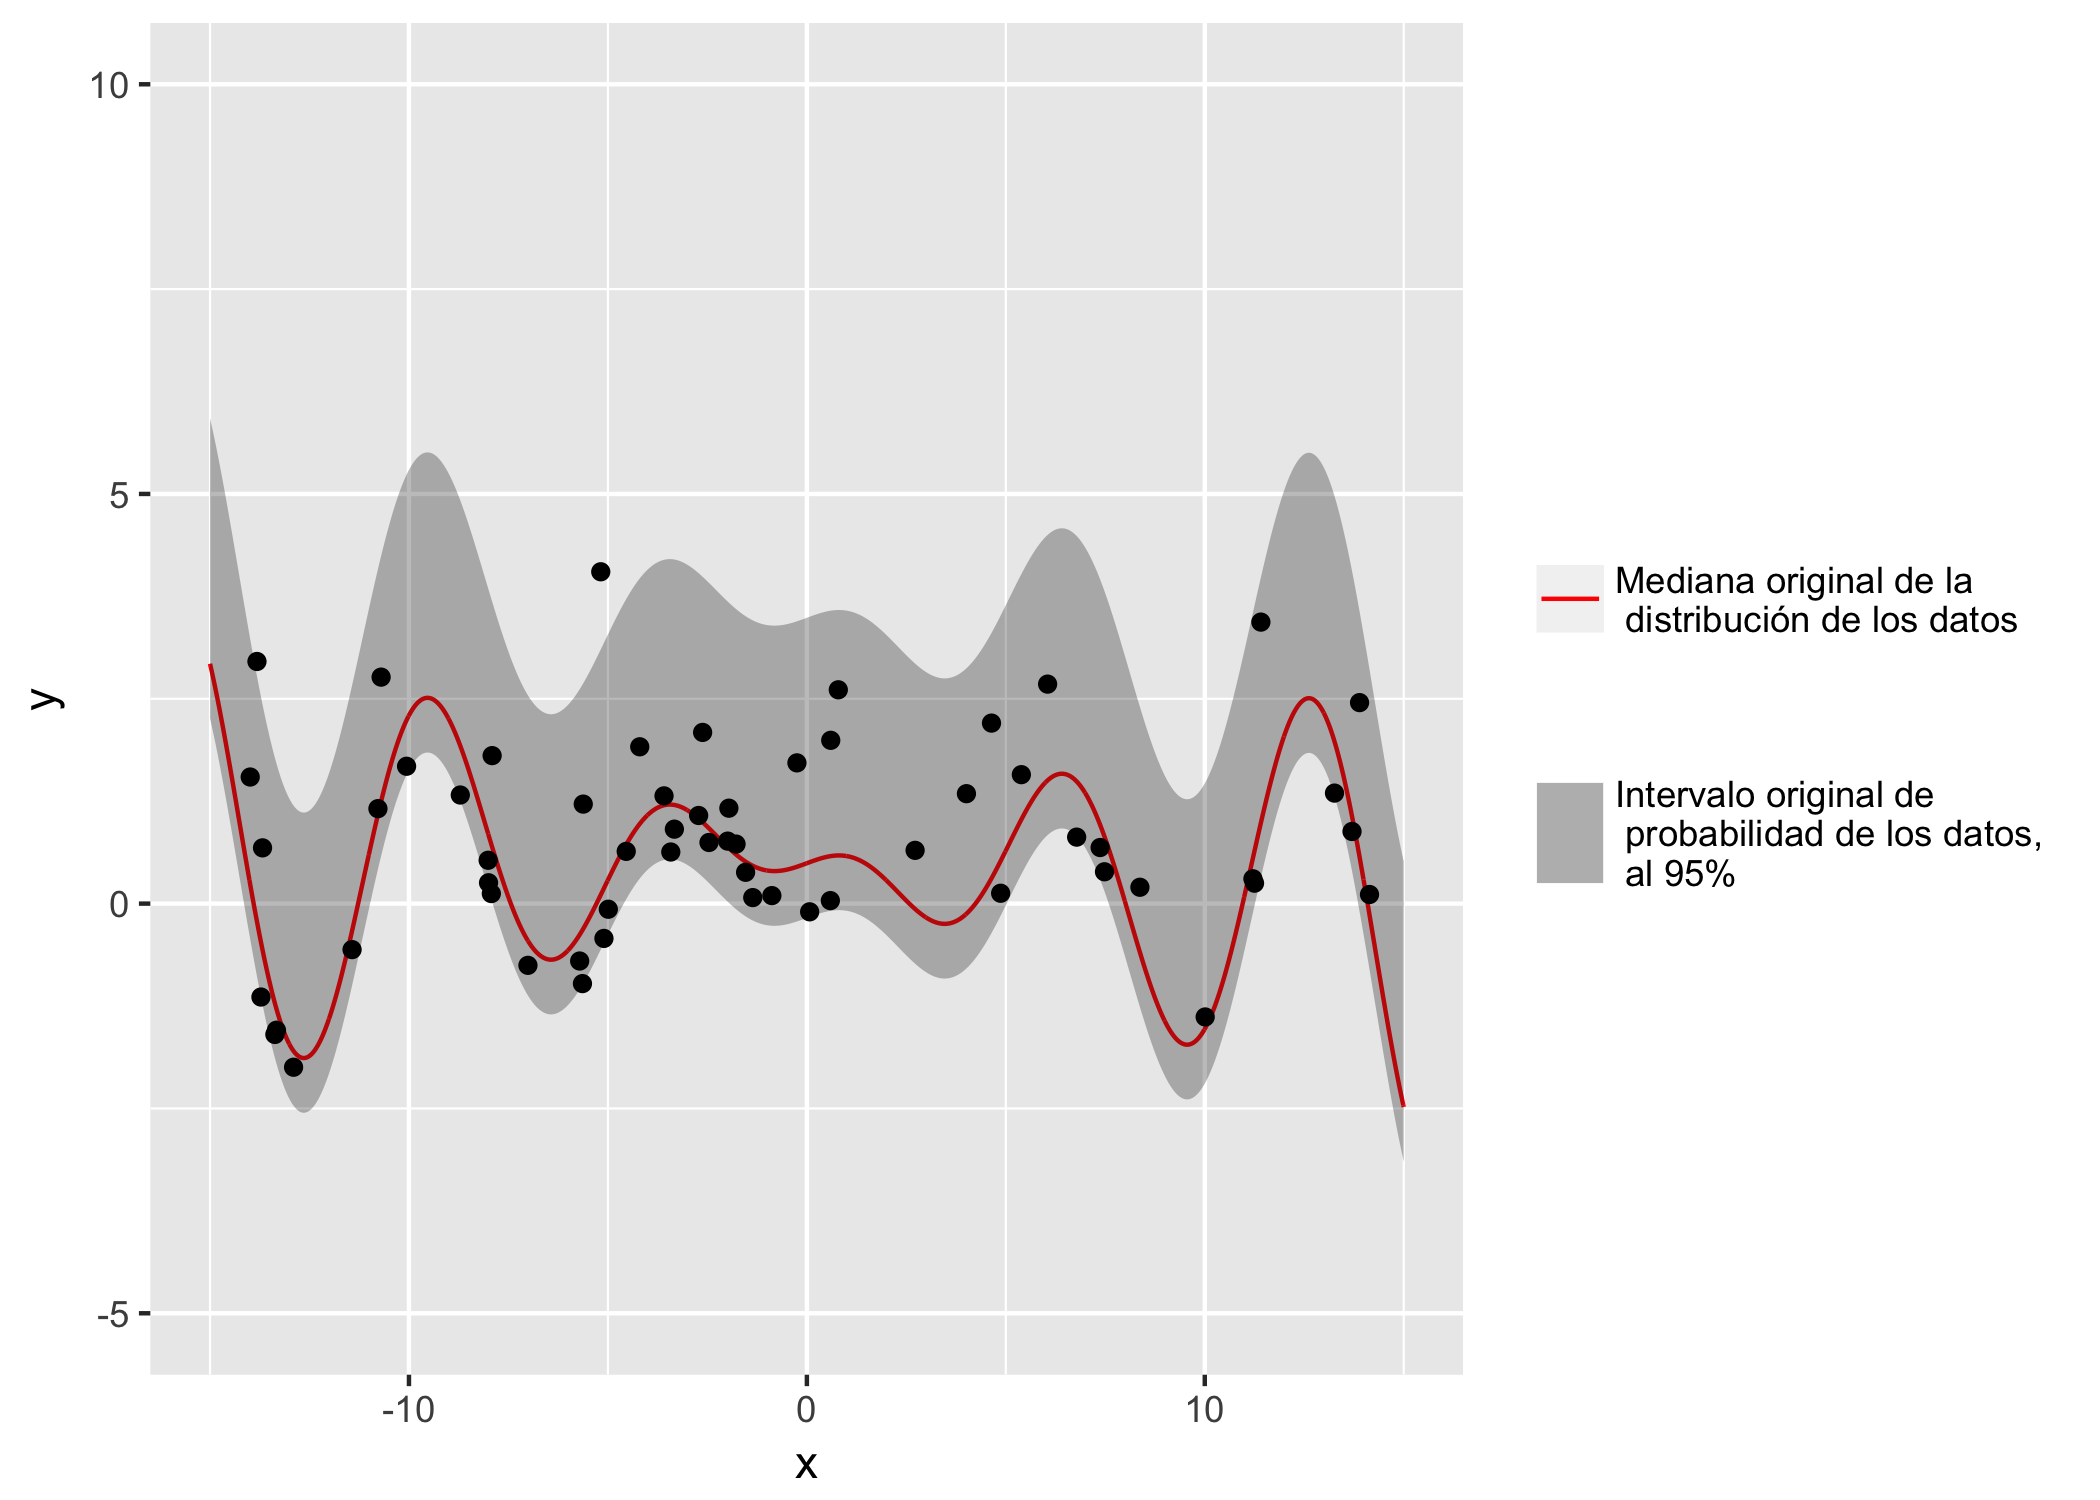
\includegraphics[width=0.7\textwidth]{Figures/Simulation/asymmetric/sample.png}
	\label{sample_asymmetric}
\end{figure}

Como se podr\'a dar cuenta el lector, la asimetr\'ia del error provoca cambios en la distancia de los cuantiles respecto a la mediana. Por dar un ejemplo, el cuantil $0.025$\textit{-\'esimo} (el l\'imite inferior del intervalo) est\'a mucho m\'as cerca de la mediana, que el cuantil $0.975$\textit{-\'esimo} (el l\'imite superior del intervalo). Esta situaci\'on es at\'ipica, ya que estamos acostumbrados a que ambos est\'en a la misma distancia, propiciado por la simetr\'ia. Por ello, es pronosticable que el modelo tradicional sufrir\'a para reflejar dicho comportamiento, debido a que supone error normal, el cual presenta la simetr\'ia a la que estamos acostumbrados. A continuaci\'on se presentan los resultados obtenidos del ajuste de ambos modelos.

\begin{table}[H]
\centering
\caption{Error cuadrático medio de datos con error asimétrico.}
\begin{tabular}{ccc}
  \hline
Cuantil & Modelo Tradicional & Modelo GPDP \\ 
  \hline
0.95 & 1.69 & 1.23 \\ 
  0.50 & 1.65 & 0.64 \\ 
  0.25 & 1.53 & 0.44 \\ 
   \hline
\end{tabular}
\label{mse_asymmetric}
\end{table}

\begin{table}[H]
\centering
\caption{Correlación al cuadrado de datos con error asimétrico.}
\begin{tabular}{ccc}
  \hline
Cuantil & Modelo Tradicional & Modelo GPDP \\ 
  \hline
0.95 & 0.00 & 0.50 \\ 
  0.50 & 0.00 & 0.61 \\ 
  0.25 & 0.00 & 0.69 \\ 
   \hline
\end{tabular}
\label{corr_asymmetric}
\end{table}

\begin{table}[H]
\centering
\caption{Porcentaje de valores reales dentro del intervalo de confianza de datos con error asimétrico.} 
\begin{tabular}{ccc}
  \hline
Cuantil & Modelo Tradicional & Modelo GPDP \\ 
  \hline
0.95 & 58\% & 100\% \\ 
  0.50 & 46\% & 100\% \\ 
  0.25 & 52\% & 100\% \\ 
   \hline
\end{tabular}
\label{within_asymmetric}
\end{table}

\begin{figure}[htbp]
	\centering
	\caption{Ajuste de los modelos Tradicional y \textit{GPDP}, para un conjunto de datos con error asim\'etrico.}
	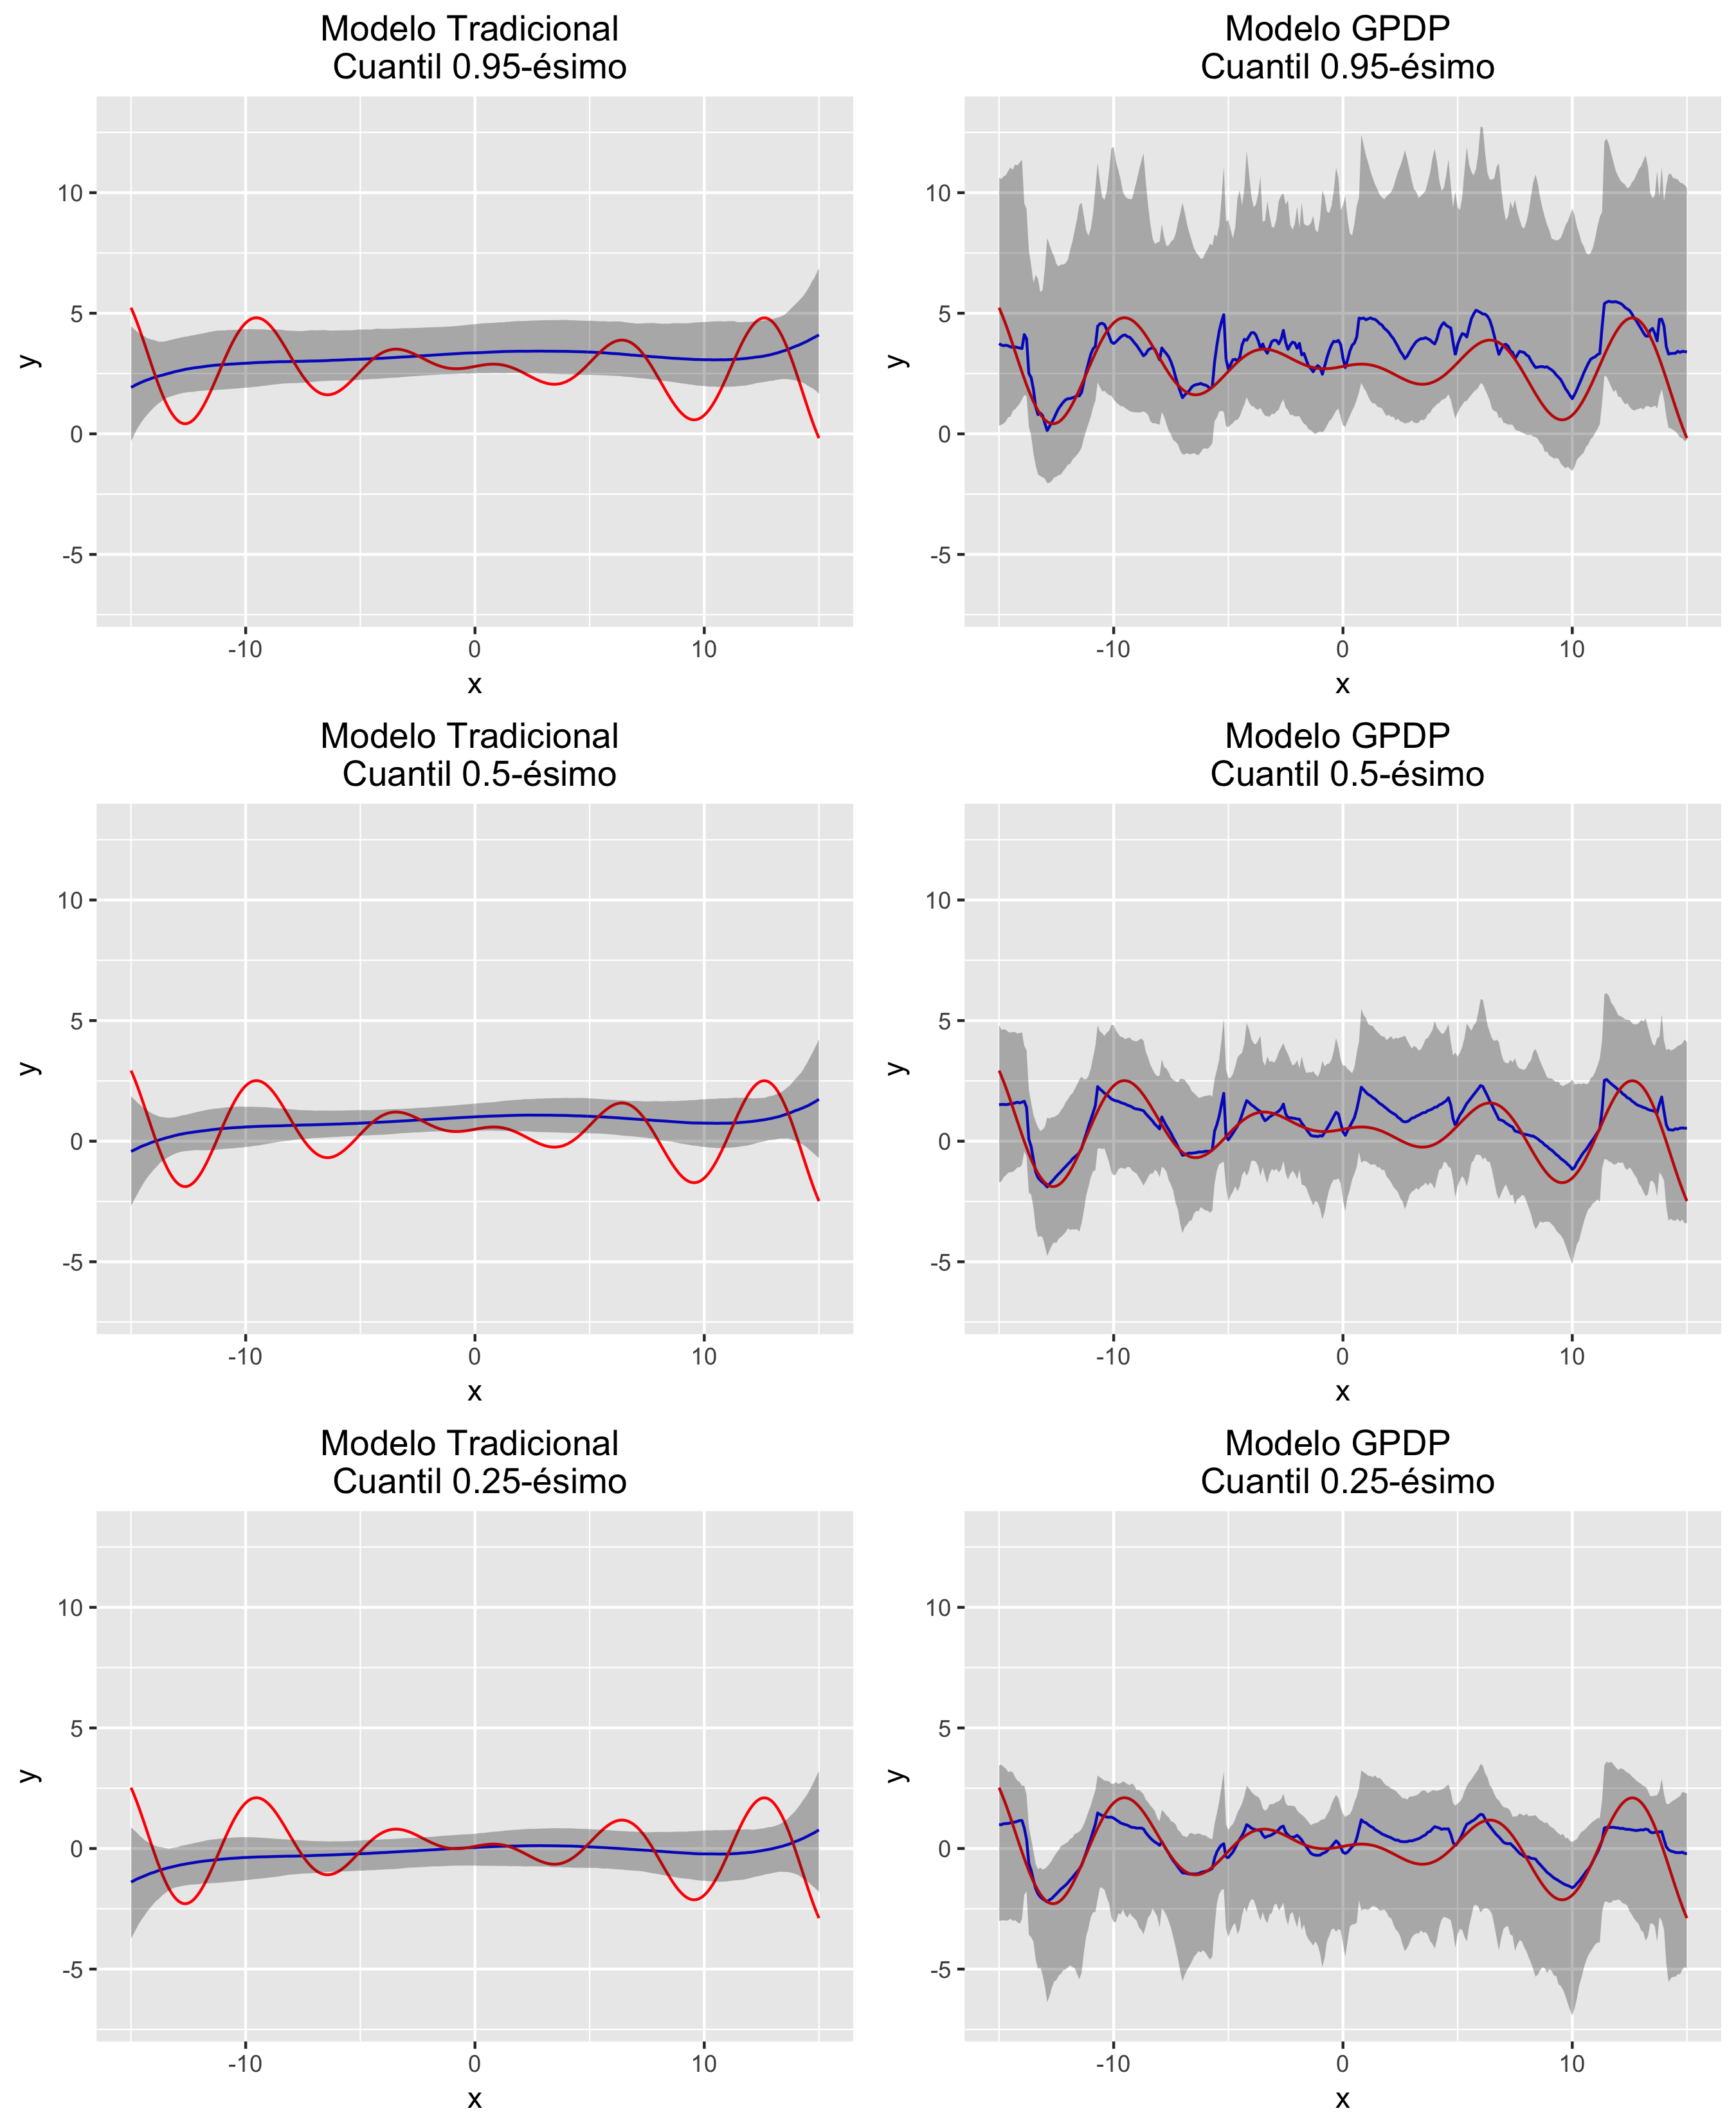
\includegraphics[width=\textwidth]{Figures/Simulation/asymmetric/predictions.png}
	\captionsetup{singlelinecheck=off,font=footnotesize}
    \caption*{Nota: La l\'inea roja representa el valor real de cada cuantil, la l\'inea azul representa la mediana de la distribuci\'on posterior predictiva y el \'area gris su intervalo de probabilidad al 95\%.}
	\label{models_asymmetric}
\end{figure}

La figura \ref{models_asymmetric} permite observar que el modelo tradicional infiere una mediana, en su mayor\'ia, mayor que la real. Esto se debe a que, por el supuesto de simetr\'ia, impl\'icitamente modela a la mediana como si fuera la media, siendo la segunda m\'as grande en su valor real, que la primera. 

La misma figura sugiere que el modelo tradicional interpret\'o a la funci\'on de los diversos cuantiles pr\'acticamente como una constante, y atribuy\'o las variaciones \'unicamente al error aleatorio. La sugerencia de la constante tambi\'en se sustenta en el cuadro \ref{corr_asymmetric}, donde es posible ver que la correlaci\'on es pr\'acticamente 0 (la primer cifra significativa es el tercer decimal), respecto a los valores originales. Adem\'as, la hip\'otesis de que las variaciones se le atribuyeron al error aleatorio se apoya en los bajos porcentajes de valores reales dentro de los intervalos de predicci\'on, presentados en el cuadro \ref{within_asymmetric}.

Por otro lado, se puede verificar en las tablas \ref{mse_asymmetric}, \ref{corr_asymmetric} y \ref{within_asymmetric} que el modelo GPDP logr\'o un mejor desempeño en todas las m\'etricas, para todos los cuantiles. Sin embargo, no hay que perder de vista que de todos los casos vistos hasta este punto, es el que present\'o intervalos de probabilidad m\'as amplios. Es decir, es el caso en el que hay mayor incertidumbre respecto a la predicci\'on. Adem\'as, present\'o niveles de correlaci\'on bajos, comparativamente hablando. No necesariamente la causa fue el error asim\'etrico, sino pudo provenir de que la forma de la funci\'on tendencia es at\'ipica y compleja de inferir para muchos modelos.

\subsection{Discontinuidades}

Dejando atr\'as las modificaciones en el error $\omega(x)$, ahora se presenta una situaci\'on at\'ipica en la funci\'on tendencia. Tanto el modelo tradicional, como el modelo GPDP, suponen continuidad en las funciones de los cuantiles. Por ello, me pareci\'o interesante averiguar c\'omo se comportar\'ia su ajuste, en caso de modelar datos que provinieran de una funci\'on tendencia discontinua. Particularmente se simul\'o utilizando la funci\'on
\begin{equation*}
g(x) = 
\begin{cases}
   - \frac{1}{5} x + 2cos(x) - 2 &\text{ si } x \in (-\infty, -5) \\
   \frac{1}{10} x^2 - \frac{1}{2}x + 1 &\text{ si } x \in [-5, 5) \\
   6 - ln(x) &\text{ si } x \in [-5, \infty)
\end{cases},
\end{equation*}
con el error t\'ipico de los modelos de regresi\'on, $\omega(x) \sim \mathcal{N}(0,1)$.

El comportamiento discontinuo se puede entender de mejor manera gr\'aficamente, como lo muestra la figura \ref{sample_discontinuous}. Adem\'as, en dicha figura tambi\'en se pueden ver los puntos obtenidos de la simulaci\'on.

\begin{figure}[H]
	\centering
	\caption{Datos simulados con discontinuidades.}
	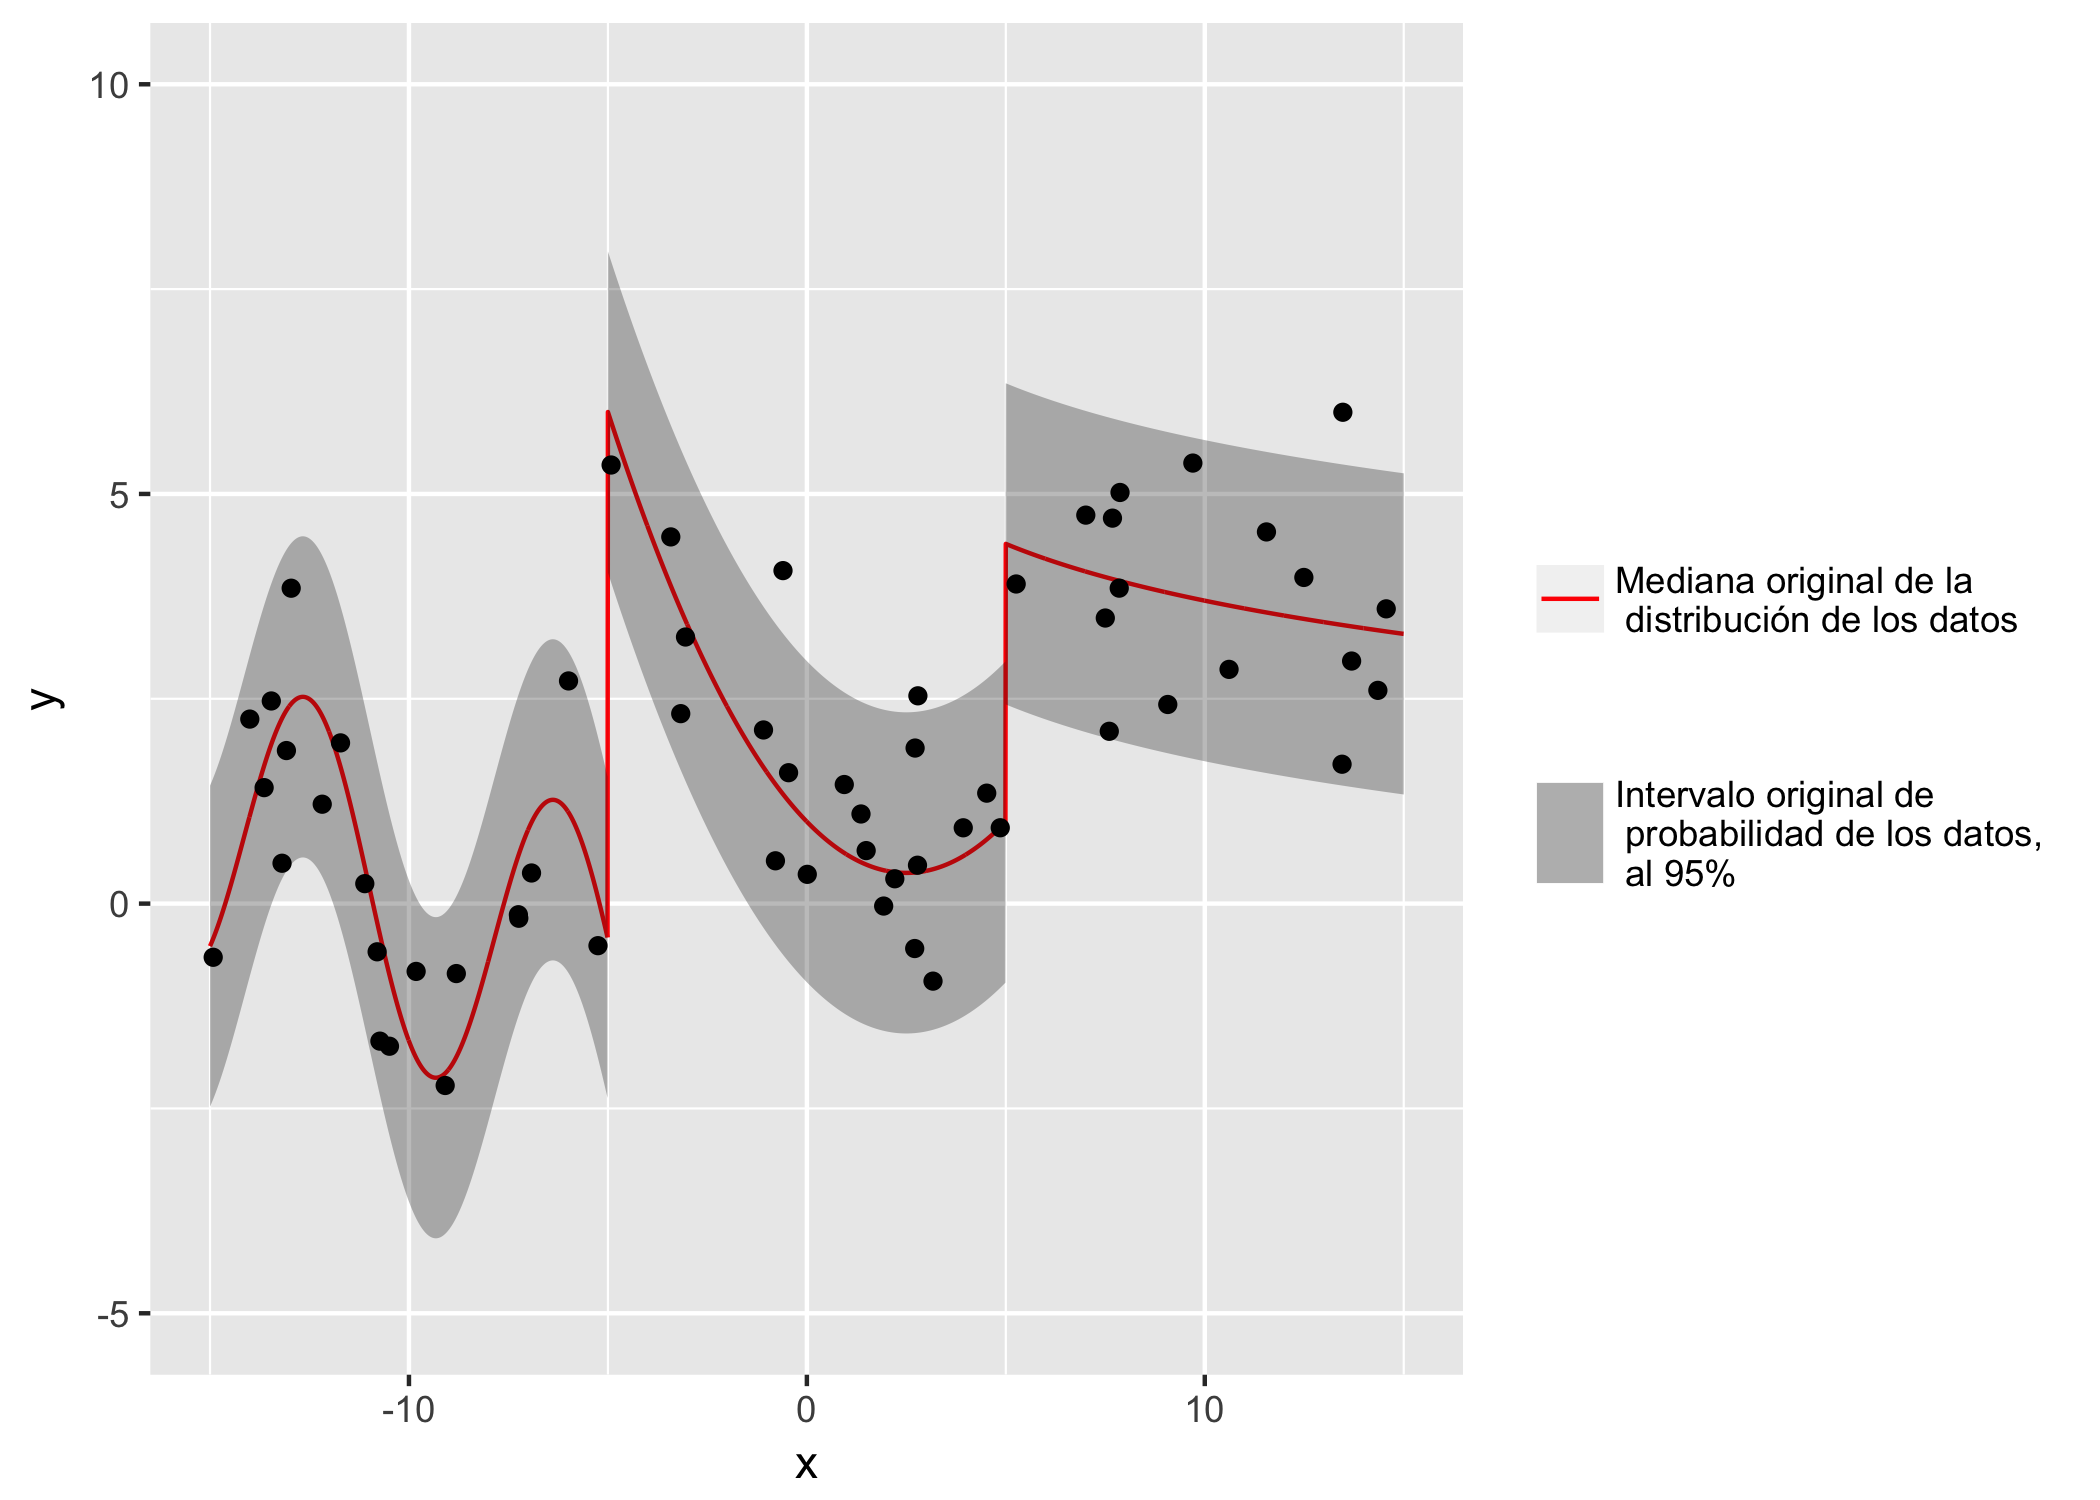
\includegraphics[width=0.7\textwidth]{Figures/Simulation/discontinuous/sample.png}
	\label{sample_discontinuous}
\end{figure}

Como se puede observar en la figura \ref{sample_discontinuous}, y en la expresi\'on matem\'atica antes mencionada, la funci\'on tendencia tiene tres secciones: la primera con un comportamiento oscilatorio, la segunda, un trozo de par\'abola, y la \'ultima, un logaritmo, que por el nivel de la covariable, asemeja a una recta. Todas, por separado, son continuas. Por lo tanto, son aproximables con polinomios en un intervalo cerrado. Sin embargo, entre cada secci\'on hay un salto de discontinuidad, por lo que la funci\'on global no puede ser expresada fielmente usando dicha familia. Ante dicha dificultad se ajustaron los modelos tradicional y GPDP, obteniendo los resultados que se presentan a continuaci\'on. 

\begin{table}[H]
\centering
\caption{Error cuadrático medio de datos simulados con discontinuidades.} 
\begin{tabular}{ccc}
  \hline
Cuantil & Modelo Tradicional & Modelo GPDP \\ 
  \hline
0.95 & 7.08 & 1.10 \\ 
  0.50 & 2.23 & 0.35 \\ 
  0.25 & 3.19 & 0.47 \\ 
   \hline
\end{tabular}
\label{mse_discontinuous}
\end{table}

\begin{table}[H]
\centering
\caption{Correlación al cuadrado de datos simulados con discontinuidades.}
\begin{tabular}{ccc}
  \hline
Cuantil & Modelo Tradicional & Modelo GPDP \\ 
  \hline
0.95 & 0.38 & 0.83 \\ 
  0.50 & 0.38 & 0.90 \\ 
  0.25 & 0.38 & 0.88 \\ 
   \hline
\end{tabular}
\label{corr_discontinuous}
\end{table}

\begin{table}[H]
\centering
\caption{Porcentaje de valores reales dentro del intervalo de confianza de datos simulados con discontinuidades.} 
\begin{tabular}{ccc}
  \hline
Cuantil & Modelo Tradicional & Modelo GPDP \\ 
  \hline
0.95 & 28\% & 98\% \\ 
  0.50 & 46\% & 100\% \\ 
  0.25 & 53\% & 99\% \\ 
   \hline
\end{tabular}
\label{within_discontinuous}
\end{table}

\begin{figure}[htbp]
	\centering
	\caption{Ajuste de los modelos Tradicional y \textit{GPDP}, para un conjunto de datos simulados con discontinuidades.}
	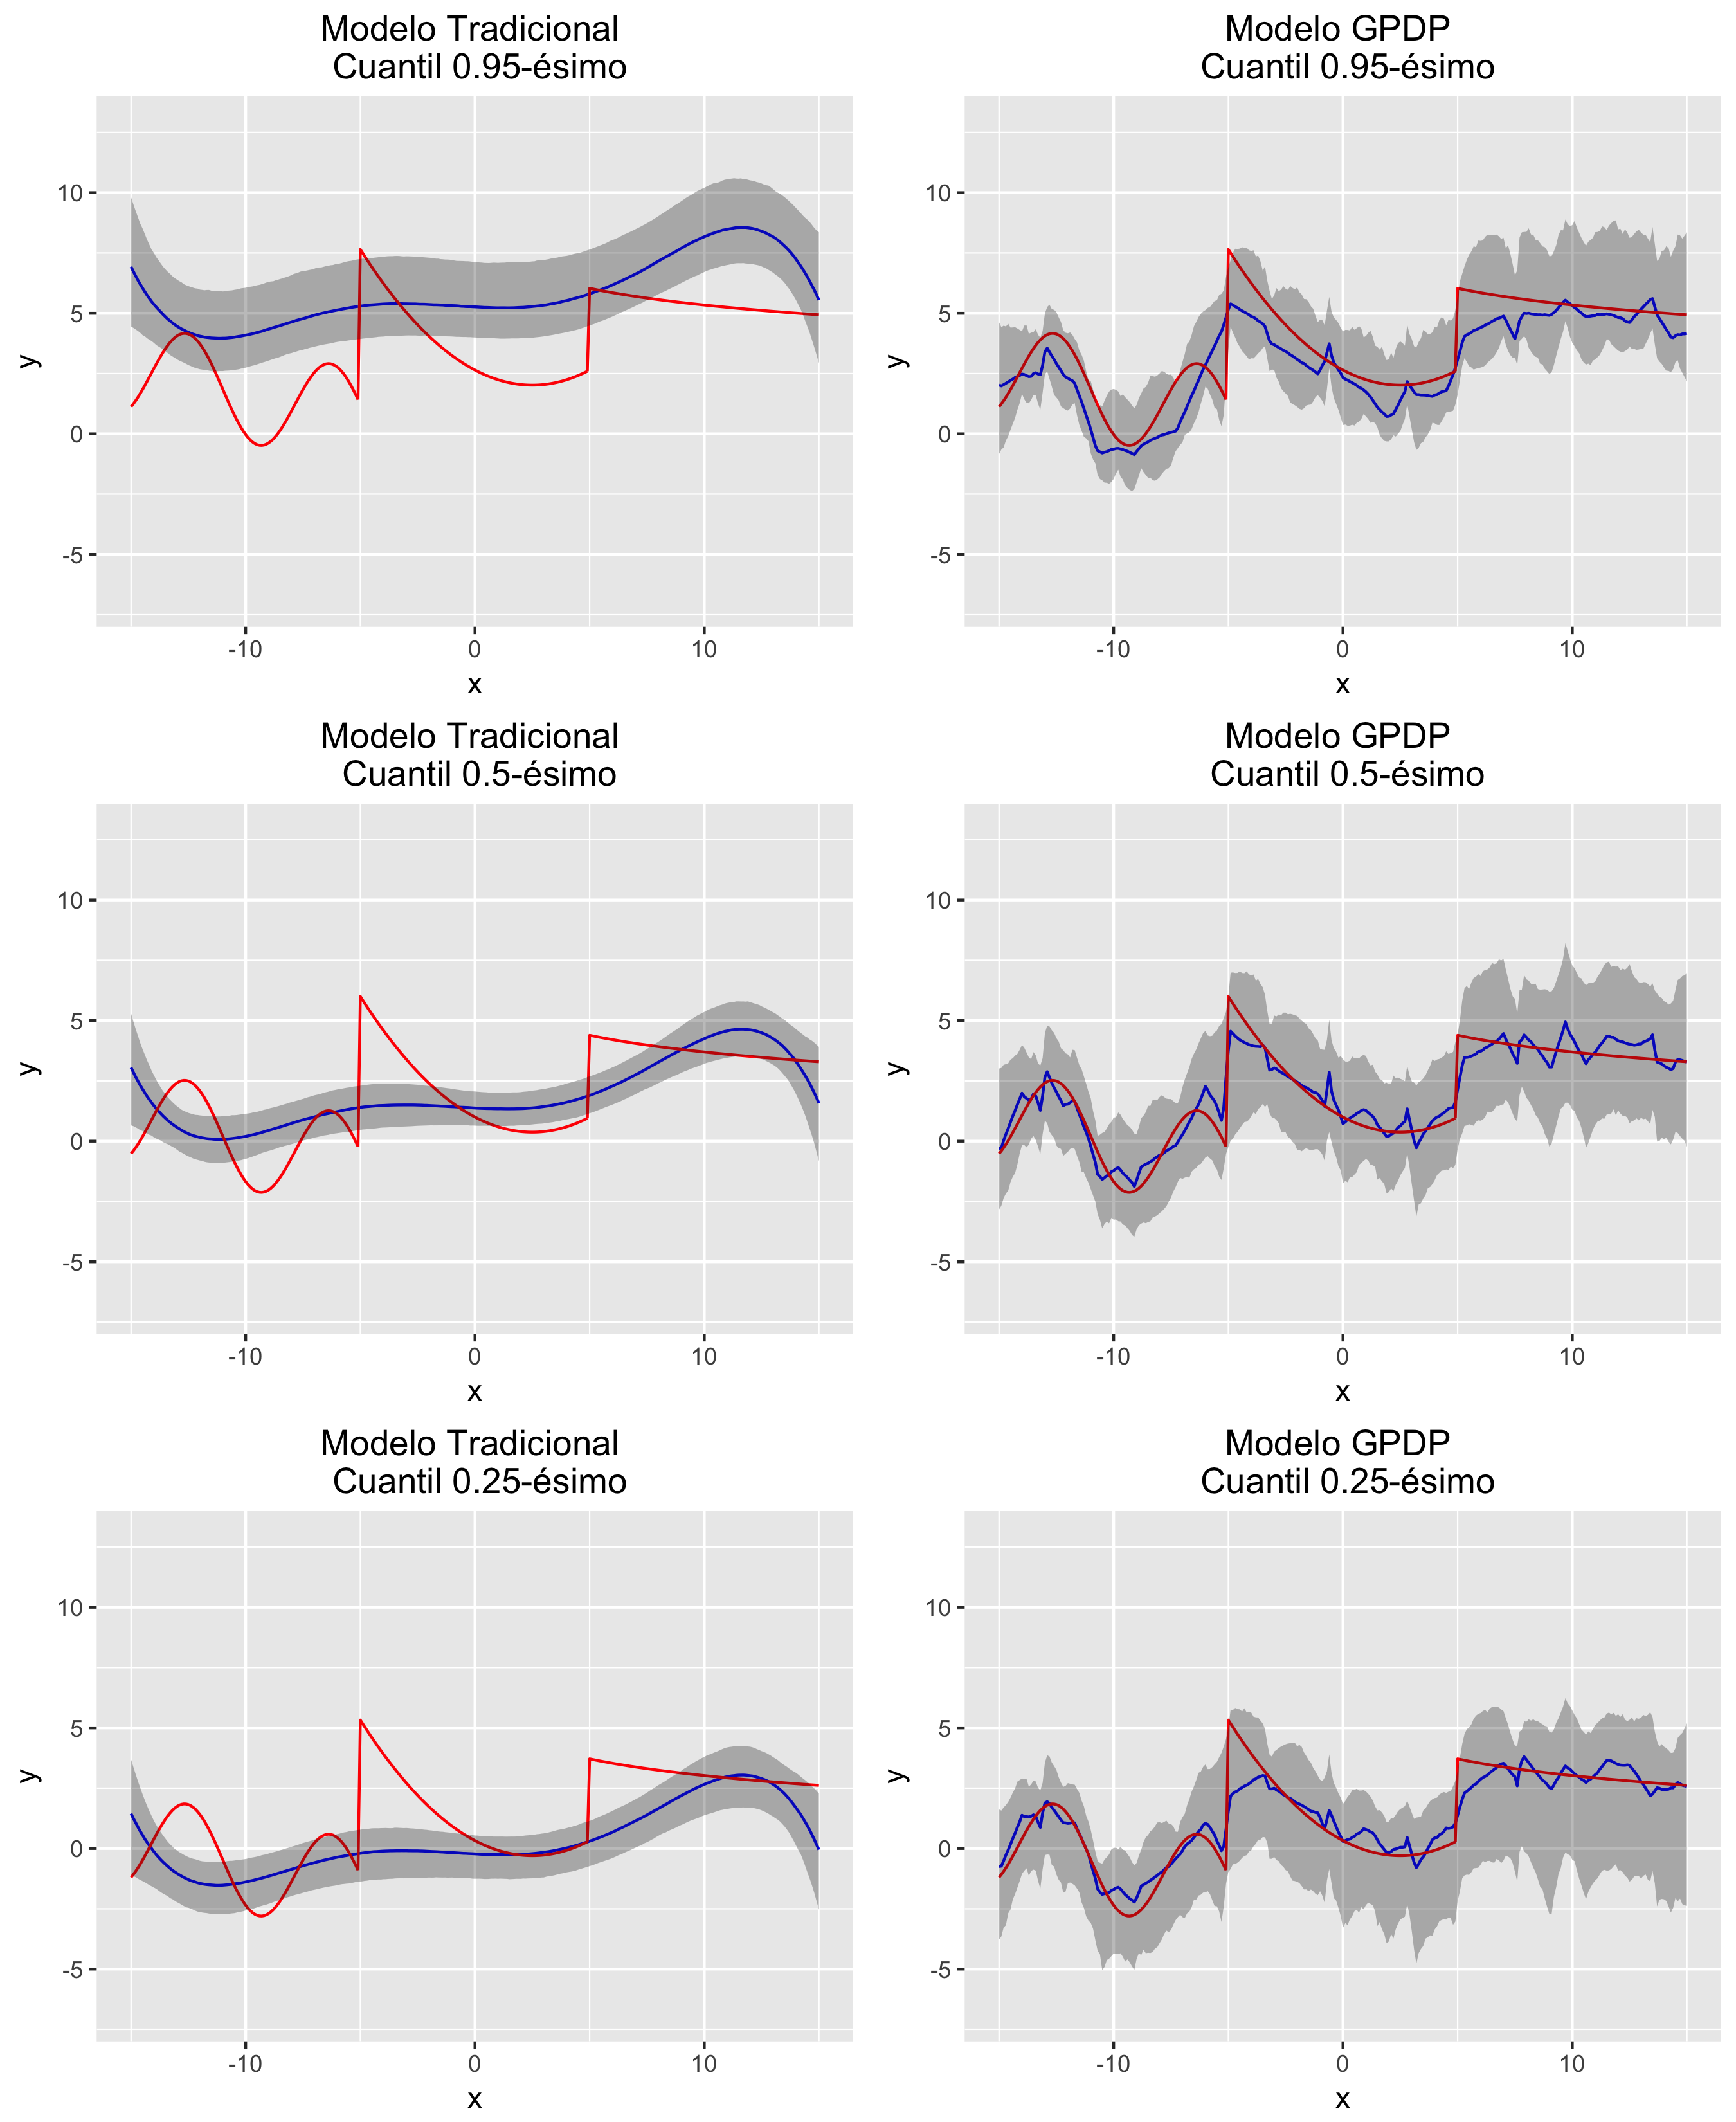
\includegraphics[width=\textwidth]{Figures/Simulation/discontinuous/predictions.png}
	\captionsetup{singlelinecheck=off,font=footnotesize}
    \caption*{Nota: La l\'inea roja representa el valor real de cada cuantil, la l\'inea azul representa la mediana de la distribuci\'on posterior predictiva y el \'area gris su intervalo de probabilidad al 95\%.}
	\label{models_discontinuous}
\end{figure}

Como se puede observar en la figura \ref{models_discontinuous}, el modelo tradicional estuvo muy lejos de inferir correctamente la forma real de la funci\'on de los distintos cuantiles. Esto tambi\'en lo confirma el cuadro \ref{within_discontinuous}, ya que en la mejor de las estimaciones del modelo tradicional, \'unicamente el $53\%$ de los datos reales se pronostic\'o dentro del intervalo de probabilidad.
Al parecer, atribuy\'o el primer salto \'unicamente al error aleatorio, el cual estim\'o de gran magnitud, raz\'on por lo que su estimaci\'on de los cuantiles $0.25$ y $0.95$\textit{-\'esimos} fue m\'as alejada de la mediana de lo que era realmente. El segundo salto parece que s\'i lo detect\'o, pero la elevaci\'on la realiz\'o paulatinamente, llegando al punto m\'aximo despu\'es de 5 unidades de donde realmente ocurri\'o.

Por otro lado, como lo confirma la exploraci\'on visual de la figura \ref{models_discontinuous}, as\'i como los cuadros \ref{mse_discontinuous}, \ref{corr_discontinuous} y \ref{within_discontinuous}, la estimaci\'on del modelo GPDP fue muy superior en calidad, debido a que tuvo errores cuadr\'aticos medios consistentemente bajos, correlaci\'on cuadr\'atica de al menos $83\%$ y al menos $98\%$ de los valores reales adentro del intervalo de probabilidad de la predicci\'on. Debido a la construcci\'on del modelo, tuvo una estimaci\'on continua de la funci\'on de los cuantiles. Sin embargo, lo compens\'o elevando r\'apidamente su nivel (dentro de vecindades m\'as pequeñas que la unidad) cuando hubo saltos de discontinuidad en la funci\'on real. Por ello, los intervalos donde la estimaci\'on fue mala fueron en realidad muy angostos.

\section{Comparaci\'on general entre modelos}
\label{models_comp}

El an\'alisis de los datos anteriores brinda informaci\'on para pensar que el ajuste del modelo GPDP fue, la mayor\'ia de las veces, igual o mejor que el del modelo tradicional de regresi\'on a la media, cuando el objetivo fue estimar el valor de los cuantiles. Esto se dio principalmente cuando se modelaron valores extremos, o los datos provinieron de situaciones que violan los supuestos de la regresi\'on tradicional a la media. 

Pasando a un an\'alisis m\'as minucioso, observ\'e detalles que considero vale la pena resaltar. Para empezar, la magnitud de los intervalos de probabilidad de predicci\'on, ya que los que present\'o el modelo GPDP fueron com\'unmente m\'as anchos que los del tradicional. Esto no significa que su estimaci\'on haya sido peor. De hecho, quiz\'as fue lo contrario. Mientras que los intervalos de probabilidad al $95\%$ del modelo GPDP siempre contuvieron, al menos, al $95\%$ de los valores reales de los cuantiles (como era esperado), hubo intervalos del modelo tradicional al $95\%$ de probabilidad que contuvieron \'unicamente al $9\%$ de los valores reales.

Hablando de los intervalos de probabilidad, es interesante observar que aquellos provenientes del GPDP se hicieron m\'as angostos, conforme hubo m\'as datos observados cercanos a ese valor, y m\'as anchos, ante la ausencia de datos en la vecindad pr\'oxima. Este comportamiento provino de la estructura de correlaci\'on dada por el proceso Gaussiano, recordando que depende de la distancia entre los datos. Por su parte, en el modelo tradicional de regresi\'on a la media, el intervalo de predicci\'on tuvo menor anchura en la parte media de los datos de $x$, y creci\'o muy ligeramente conforme se acerc\'o a los valores m\'inimo y m\'aximo observados. En lo personal, prefiero el comportamiento del modelo GPDP, ya que considero que entre mayor sea la cantidad de datos cercanos, se deber\'ia tener menor incertidumbre, y viceversa.

Tambi\'en es interesante observar que la mediana de la predicci\'on en el modelo tradicional se encontr\'o usualmente en medio del intervalo. Por otro lado, debido a que supone que el error es una mezcla infinita de procesos de Dirichlet, el modelo GPDP present\'o, en algunos casos, asimetr\'ia en la distribuci\'on posterior predictiva.

Las personas que hemos trabajado con el modelo tradicional de regresi\'on a la media estamos acostumbrados a que cualquier estimaci\'on puntual que tomemos es suave, ya que se puede expresar como polinomio, y, por lo tanto, es infinitamente diferenciable. En cambio, debido a los supuestos que introduce el modelo GPDP para el proceso Gaussiano, sus estimaciones puntuales mantuvieron un comportamiento mucho menos suave, pero que fue \'util para capturar cambios bruscos en la funci\'on. Sin embargo, es importante recordar que la dificultad de interpretaci\'on que tienen los modelos no param\'etricos representa una de sus mayores desventajas.

Finalmente, es interesante comparar la diferencia en tiempos de ajuste y predicci\'on para ambos modelos, los cuales se muestran en las figuras \ref{fit_time} y \ref{pred_time}. \footnote{Estos tiempos se obtuvieron corriendo los procesos en una MacBook, con procesador 1.1 GHz Intel Core M, y memoria RAM DDR3, de 8 GB y 1600 MHz. Los procesos de predicci\'on se corrieron en paralelo, usando 2 de los 4 núcleos.} Cabe señalar que los tiempos presentados son el acumulado de ajustar o predecir los modelos de los tres cuantiles.

\begin{table}[H]
\centering
\caption{Tiempo de ajuste por conjunto de datos, para cada modelo.} 
\begin{tabular}{ccc}
  \hline
Datos & Tradicional (seg) & GPDP (seg) \\ 
  \hline
Supuestos tradicionales & menos de 1 & 2,498 \\ 
  Colas pesadas & menos de 1 & 4,006 \\ 
  Heterocedasticidad & menos de 1 & 3,502 \\ 
  Error asimétrico & menos de 1 & 6,707 \\ 
  Discontinuidades & menos de 1 & 3,062 \\ 
   \hline
\end{tabular}
\label{fit_time}
\end{table}

\begin{table}[H]
\centering
\caption{Tiempo de predicción por conjunto de datos, para cada modelo.} 
\begin{tabular}{ccc}
  \hline
Datos & Tradicional (seg) & GPDP (seg) \\ 
  \hline
Supuestos tradicionales & 6.4 & 563.8 \\ 
  Colas pesadas & 4.7 & 529.0 \\ 
  Heterocedasticidad & 5.3 & 534.5 \\ 
  Error asimétrico & 5.7 & 537.4 \\ 
  Discontinuidades & 5.0 & 533.2 \\ 
   \hline
\end{tabular}
\label{pred_time}
\end{table}

Analizando los tiempos de ajuste, y recordando que se usaron 60 datos en todos los casos, es clara la bondad dada por la propiedad conjugada del modelo tradicional. \'Esta permite obtener una expresi\'on anal\'itica cerrada para la distribuci\'on posterior de los par\'ametros, y por ende, el ajuste consiste \'unicamente en multiplicaciones matriciales que toman menos de un segundo. Adem\'as, por las caracter\'isticas de este modelo, \'unicamente se requiri\'o ajustar una vez por conjunto de datos, independientemente de que se usara para varios cuantiles.

Por otro lado, el modelo GPDP requiere un ajuste distinto por cuantil, y el tiempo que tarda en correr est\'a siempre en funci\'on de la cantidad de iteraciones que se eligen realizar. En el caso particular de este trabajo, se corrieron 20,000 iteraciones para todos los casos, lo cual representa un n\'umero poco sobresaliente, comparado con las que normalmente se utilizan cuando se busca tener una precisi\'on alta. El modelo que menos tard\'o requiri\'o m\'as de 40 minutos para realizar el ajuste, por lo que la diferencia es abismal entre ambos modelos.

De hecho, es interesante ver c\'omo hay grandes diferencias dentro de los propios ajustes del modelo GPDP. La raz\'on principal es la simulaci\'on de una distribuci\'on normal truncada en cada iteraci\'on del algoritmo, usando un m\'etodo de aceptaci\'on y rechazo. Cuando los datos cumplieron los supuestos tradicionales, fue cuando le cost\'o menos trabajo realizar las simulaciones. En cambio, cuando se us\'o una funci\'on con muchas subidas y bajadas, y error asim\'etrico, el algoritmo requiri\'o m\'as del doble de tiempo para poder ajustar el modelo.

Para el caso de las predicciones, el n\'umero de puntos aument\'o a 300 para todos los casos. Sin embargo, debido a que estas simulaciones ya no pertenecen a una cadena de Markov, se pueden correr en paralelo para los dos modelos. Ambos requieren simular una distribuci\'on Normal, pero el tradicional simula una marginal por cada dato, mientras que el GPDP requiere simular una conjunta, de dimensi\'on igual al n\'umero de datos. Esa es la raz\'on por la que tarda 100 veces m\'as.

As\'i, mientras que el modelo GPDP mostr\'o, en general, mejores resultados en la precisi\'on, el modelo tradicional de regresi\'on a la media fue mucho m\'as efectivo en tiempo. Por ello, el modelador deber\'ia considerar cu\'al de ambas prefiere en su estudio, para poder tomar una mejor decisi\'on de qu\'e modelo elegir.


\newpage